\documentclass[reqno,12pt,oneside]{report} % right-side equation numbering, 12 point font, print one-sided
%\documentclass[reqno,12pt,twoside,openright]{report} % right-side equation numbering, 12 point font, print two-sided, Chapters start on odd pages. Rackham only accepts one-sided, so this is for personal printings.

\usepackage{rac}         % Use Rackham thesis style file
\usepackage[hyphens]{url}
\usepackage{lipsum}
\usepackage{graphicx}
\usepackage{todonotes}
%% Tentative: newtx for better-looking Times
\usepackage[utf8]{inputenc}
%\usepackage[T1]{fontenc}
\usepackage{newtxtext,newtxmath}

%\usepackage{aas_macros}  % To allow the reading of ADS journal references in the bibliography
\usepackage{amsmath} % Puts the limits of integrals on top and bottom
\usepackage{amsxtra}     % Use various AMS packages
%\usepackage{amsthm,bbold}
\usepackage{amssymb,fixmath}
\usepackage{amsfonts}
\usepackage{nicefrac}    % Add some packages for figures. Read epslatex.pdf on ctan.tug.org
\usepackage{rotating}
\usepackage{color}
\usepackage{epsfig}
%\usepackage{subfigure}   % To make subfigures. Read subfigure.pdf on ctan.tug.org
\usepackage{verbatim}
\usepackage[printonlyused]{acronym} % For the List of Abbreviations. Read acronym.pdf on ctan.tug.org
\usepackage{algpseudocode}
\usepackage{algorithm}

\usepackage[]{hyperref}	
\usepackage{verbatim}
\usepackage{braket,float}
\usepackage{pdflscape,everypage}
\usepackage[inline]{enumitem}
\usepackage{mathtools}
\usepackage{nomencl}
\makenomenclature

\usepackage{setspace}    % Allows you to specify the line spacing
\doublespacing           % \onehalfspacing for 1.5 spacing, \doublespacing for 2.0 spacing.
%%%%%%%%%%%%%%%%%%%%%%%%%%%%%%%%%%%%%%%%%%%%%%%%%%%%%%%%%%%%%%%%%%%%%%%%%%%%%%%

%\numberwithin{theorem}{chapter}     % Numbers theorems "x.y" where x
                                    % is the section number, y is the
                                    % theorem number

%\renewcommand{\thetheorem}{\arabic{chapter}.\arabic{theorem}}

%\makeatletter                      % This sequence of commands will
%\let\c@equation\c@theorem          % incorporate equation numbering
%\makeatother                       % into the theorem numbering scheme

%\renewcommand{\theenumi}{(\roman{enumi})}

%%%%%%%%%%%%%%%%%%%%%%%%%%%%%%%%%%%%%%%%%%%%%%%%%%%%%%%%%%%%%%%%%%%%%%%%%%%%%%


% If printing two-sided, this makes sure that any blank page at the
% end of a chapter will not have a page number.
\makeatletter
\def\cleardoublepage{\clearpage\if@twoside \ifodd\c@page\else
\hbox{}
\thispagestyle{empty}
\newpage
\if@twocolumn\hbox{}\newpage\fi\fi\fi}
\makeatother


%%%%%%%%%%%%%%%%%%%%%%%%%%%%%%%%%%%%%%%%%%%%%%%%%%%%%%%%%%%%%%%%%%%%%%%%%%%%%%%
%%% The following is needed so that the pagenumber 
%%% in the landscape mode appears in the right place
%%%%%%%%%%%%%%%%%%%%%%%%%%%%%%%%%%%%%%%%%%%%%%%%%%%%%%%%%%%%%%%%%%%%%%%%%%%%%%%
\newcommand{\Lpagenumber}{\ifdim\textwidth=\linewidth\else\bgroup
  \dimendef\margin=0 %use \margin instead of \dimen0
  \ifodd\value{page}\margin=\oddsidemargin
  \else\margin=\evensidemargin
  \fi
  \raisebox{\dimexpr -\topmargin-\headheight-\headsep-0.5\linewidth}[0pt][0pt]{%
    \rlap{\hspace{\dimexpr \margin+\textheight+\footskip}%
    \llap{\rotatebox{90}{\thepage}}}}%
\egroup\fi}
\AddEverypageHook{\Lpagenumber}%

%%%%%%%%%%%%%%%%%%%%%%%%%%%%%%%%%%%%%%%%%%%%%%%%%%%%%%%%%%%%%%%%%%%%%%%%%%%%%%

%% Uncomment if using Bib-tex
% \usepackage[authoryear,sort&compress]{natbib}
% \usepackage{bibunits}
% \defaultbibliographystyle{apsrmp}
% \usepackage{babel,csquotes,xpatch}% recommended

% Must use biblatex to produce the Published Contents and Contributions, per-chapter bibliography (if desired), etc.
\usepackage[backend=biber,natbib,style=phys,url=false,giveninits=true,uniquename=false, hyperref]{biblatex}
\addbibresource{References.bib}



%%%%%%%%%%%%%%%%%%%%%%%%%%%%%%%%%%%%%%%%%%%%%%%%%%%%%%%%%%%%%%%%%%%%%%%%%%%%%%%
\begin{document}


% Title page as required by Rackham dissertation guidelines
\titlepage{Electronic Spectroscopy of Topological Superconductor FeTe$_{0.55}$Se$_{0.45}$}{Mason J. Gray}
{Doctor of Philosophy}{May}{2021}

% Begin the front matter as required by Rackham dissertation guidelines
\initializefrontsections

% Optional Frontispiece
%\frontispiece{\includegraphics[width=\textwidth]{Intro/Frontispiece.png}}

% Optional, but recommended, Copyright page
\copyrightpage{2021}{Mason J. Gray}

% Page numbering. If you don't include a frontispiece or copyright page, you'll need to change this for two-sided printing.
\makeatletter
\if@twoside \setcounter{page}{4} \else \setcounter{page}{1} \fi
\makeatother

% Optional in-dissertation Abstract Page
\startabstractpage
{Electronic Spectroscopy of Topological Superconductor FeTe$_{0.55}$Se$_{0.45}$}{Mason J. Gray}{Kenneth S. Burch, Ph.D.}
In condensed matter physics we study the behavior of crystals at finite density and low temperatures. By tuning and breaking the various materials, symmetries, and the topology of a crystal one can bring about brand new quantum phases of matter. These new phases of matter in turn produce emergent quasiparticles such as the cooper pair in superconductivity, the spinon in magnetic systems, and the Fermi arcs in Weyl semimetals. \par
Of particular interest are systems in which superconductivity interacts with topology. These systems have been theoretically predicted to produce anyonic quasiparticles which may be used as qubits in a future fault-tolerant quantum computer. However, these system usually require the use of the superconducting proximity effect to inject cooper pairs into the topological system. This is turn requires interfacing two different materials which not only requires extremely clean interfaces, but also matching Fermi surfaces, comparable Fermi velocities, and more. The ideal candidate for topological superconductivity would therefore be a material that is both superconducting and topologically non-trivial. One promising candidate is the iron-based superconductor FeTe$_{(1-x)}$Se$_{x}$, specifically the at \ac{FTS} doping  which also has non-trivial topology. In this dissertation we address the fabrication of pristine interfaces using a new tool as well as new probes into the topology of \ac{FTS}.\par
In Chapter II we discuss the motivation, construction, and use of the ``cleanroom-in-a-glovebox". 
This tool places an entire nanofabrication workflow into an inert argon atmosphere which has allowed us access to study a myriad of new materials and systems. A delightful offshoot of this glovebox is that it is a useful tool in training new scientists in fabrication techniques. The photolithography, \ac{PVD}, and characterization tools in the glovebox are designed to be easy to use and thus afford new users a low-risk method of learning new techniques.\par
In chapter III we discuss a specific example of a new quantum phase of matter e.g. topological superconductivity in FTS. There, I discuss the fabrication requirements to probe this elusive phase as well as the unique measurement technique used to provide evidence that FTS is a higher-order topological superconductor. The characterization of FTS continues in Chapter IV where we reveal some exciting new results in the \ac{FTS} system. These new results are direct evidence for the topological nature of \ac{FTS}, a feat which has only been shown in \ac{ARPES} and \ac{STM}\par
Chapter V concludes the dissertation with a summary of Chapters II, III, and IV. In addition, we give suggestions for future experiments to investigate the FTS system further as well as suggestions for insightful teaching programs with the cleanroom-in-a-glovebox.
\label{Abstract}

% Optional Dedication page
%\dedicationpage{For my family and my loving, supporting wife, Amanda.}

% Optional Preface page
%\startprefacepage
%\input{Preface}
%\label{Preface}

% Table of contents, list of figures, etc.
\tableofcontents     % Required
\listoffigures       % Required if there is more than one figure
%\listoftables        % Required if there is more than one table
%\listofmaps          % Required if there is more than one map
%\listofappendices    % Required if there is more than one appendix
\listofabbreviations % Optional. Abbreviations should be stored in a file named abbr.tex

% Optional Acknowledgements page
\startacknowledgementspage
To start I would like to extend my deepest gratitude to my advisor, Prof. Kenneth S. Burch. Through many difficult assignments and tasks (some that I was convinced were impossible before trying) I have grown quite a bit since my first days in your lab building a transfer stage. Thank you for helping me become a better scientist, writer, and communicator. But more so thank you for being a mentor. \par
I would also like to thank the professors who graciously served on my dissertation committee: Professor Qiong Ma, Professor Brian Zhou, and Professor Ying Ran. I have learned quite a lot from all of you, your works, and your physics talks. I continue to be inspired by the science produced from your groups everyday. Thank you for being a role model.\par
I am extremely grateful to have had lab-mates as skilled and fun as those in LASE. The constant conversations ongoing in the lab have greatly extended my understanding of physics, chemistry, and even biology. I continue to be flabbergasted by the results produced out of the cleanroom-in-a-glovebox and I know I leave it in good hands. I would like to extend a particular thank you to a previous LASE member, Gavin Osterhoudt, for many late nights and weekends spent debating physics, MatLab, LabView, pizza, beer, and the danger levels posed by each family of animal. Thank you for the laughs!\par
In addition, I am also thankful to all of my wonderful collaborators. Your projects and papers have really made the glovebox shine in a way that would be simply impossible without you. \par
I would like to extend a thank you to the whole physics graduate student body at Boston College for making the building positive and fun. I would like to extend a special thanks to Matthew Gochan for making sure that I keep my mind and body in healthy shape. \par
I extend my thanks to the administrative staff of the Boston College physics department, Scott Bortolotto, Nancy Chevry, Jane Carter, and (formerly) S\'{i}le N\'{i} Scanl\'{a}in. The department simply would not run without you.\par
Apart from the scientific community, I want to thank my family for helping me through all the trials and tribulations of graduate school. The video and phone calls ensured that I was never too far from home.\par
I would like to thank all of my friends who have been so supportive over the last few years: Kyle, Lucas, Phil, Garrett, Glenna, Rutger, Fresca, Pippin, Gizmo, Naga, Rosa, and Lexington.\par
Lastly, I of course must thank my beautiful wife, Amanda. I could not have done this without you. 
\label{Acknowledgements}

\startthechapters
% The individual files for each of the chapters are put here.
% Save each chapter of your thesis to a separate tex file
% and then use the \input command to include this file in your
% thesis.  For instance you can save a file to "intro.tex" and
% then type \input{intro}.

\chapter{Introduction}
\label{chap:Intro}
At the beginning of the 20$\textsuperscript{th}$ century the world underwent the first quantum revolution. New ideas about wave-particles duality and quantization gave scientists the tools to explain previously observed phenomena such as the periodic table. With a deeper understanding, this new quantum theory drove revolutionary technologies such as electronic semiconductors thus bringing the world into the Information age. Now we are undergoing a second quantum revolution where we are no longer using quantum mechanics to simply explain observed phenomena, we are actively \textit{controlling} quantum mechanics.\cite{Dowling2003} We are using quantum technologies to organize and build complex systems at the atomic level. This extraordinary leap forward has allowed us to create and research new quantum phases of matter and their associated new quasi-particles. Aside from the importance of understanding novel fundamental physics, research into new quantum phases of matter is paramount for driving new technologies forward. For example, research into high-temperature superconductivity may lead us to room-temperature superconductivity, a phenomena which would massively reduce energy dissipation in modern electronics. In this dissertation, we describe the development of new equipment to help build these new quantum tools as well as the novel iron-based topological superconducting system such equipment has allowed us to probe.
\section{Scope}
The works presented in this dissertation fall into two main parts: advances in nano-fabrication equipment and topological superconductivity. The first part introduces recent advances in condensed matter physics along with the difficulties associated with fabricating electronic devices to better study these new topics. In particular, we discuss materials that are acutely air-sensitive such as GdTe$_{3}$ as well as materials that are stable in air but have air-sensitive surfaces such as \ac{FTS}. The second part dives into the subject topological superconductors and higher order topology. Specifically, we focus on the iron-based superconductor \acl{FTS}, its topological properties, and some exciting new experiments.\par
The rest of this introduction will review pertinent background material. We introduce the notion of emergence and quantum phases of matter with specific applications to superconducting materials. We will leave some of the more advanced subjects of superconductivity, e.g. tunneling into a superconductor from a normal metal, to the appendices where these subjects can get a more in-depth treatment. A brief overview of topology will be given but more focus will be spent on how to treat the notion of topology in superconductivity.
\section{Emergence and New Phases of Matter}
Emergence can be colloquially summarized as, ``The whole is greater than the sum of its parts." Examples of emergence are all around us from the biggest of scales where galaxies coalesce into superclusters to the smallest of scales where atoms emerge out of the fundamental excitations of quantum fields. With such a huge subject it may be difficult to see how this concept is useful in driving a research direction. Thus to keep this work on track we will use the sharper definition provided by Kivelson \& Kivelson:
\begin{quote}
	``An emergent behavior of a physical system is a qualitative property that can only occur in the limit that the number of microscopic constituents tends to infinity."\cite{Kivelson2016}
\end{quote}
Using this definition, it is evident that emergence heavily influences condensed matter systems. Indeed, phases of matter are a prime example of emergence as a single crystal can exhibit wildly different properties depending on \textit{external} conditions.
\par 
Many of these phases of matter can be described elegantly through the language of symmetry and symmetry breaking\cite{Noether1918, Landau1937, pathria_beale_2022}. Quantum Hall Effect. Symmetry cannot explain everything. Topology! Berry Phase! Using symmetry and topology together we can fabricate awesome new phases with new quasiparticles. Example above the new quasiparticle is the 1D dispersionless edge mode. 
\section{Topological Superconductivity}
Smooth transition from general topology to topological superconductivity in particular. Topological superconductivity 
An in-depth derivation of the \ac{BdG} equations for superconductivity are presented in Appendix \ref{app:ARfit}, here we will use the final Hamiltonian from that appendix with some minor alterations. We will be closely following the works of Kitaev and Bernevig \& Hughes\cite{Kitaev2001, bernevig_hughes_2013}.\par 
We begin by describing a 1-D chain of fermions, i.e., at each lattice site $j$ on the chain there is a complex fermion $c_{j}$. For simplicity, we consider these complex fermions to either be spinless or fully spin-polarized due to a source of time-reversal symmetry breaking. Since a momentum-independent s-wave pairing potential is not possible for spinless fermions, we will use a momentum-dependent p-wave potential (in momentum space):
\begin{align}
	H_{\Delta} = \frac{1}{2}\left(\Delta pc_{p}^{\dagger}c_{-p}^{\dagger}+\Delta^{*}pc_{-p}c_{p}\right)
\end{align}
where $c^{\dagger}$ and $c$ are the creation and annihilation operators, $p$ is the momentum, and $\Delta$ is the superconducting pairing potential. The lattice \ac{BdG} Hamiltonian (in real space) we need to solve is:
\begin{align}
	H_{BdG} = \sum_{j}\left[-t\left(c_{j}^{\dagger}c_{j+1}+c_{j+1}^{\dagger}c_{j}\right)-\mu c_{j}^{\dagger}c_{j}+|\Delta|\left(c_{j+1}^{\dagger}c_{j}^{\dagger}+c_{j}c_{j+1}\right)\right]
\end{align}
where $t>0$ is the hopping parameter and $\mu$ is the chemical potential. To investigate how each parameter affects the superconducting gap, we take a lattice Fourier transform to convert back into momentum space:
\begin{align}
	H_{BdG} = \frac{1}{2}\sum_{p}\Psi_{p}^{\dagger}
	\begin{pmatrix}
		-2t\cos(p)-\mu & 2i|\Delta|\sin(p)\\
		-2i|\Delta|\sin(p) & 2t\cos(p)+\mu
	\end{pmatrix}
	\Psi_{p}
\end{align}
where $\Psi_{p}=(c_{p}\quad c_{-p^{\dagger}})$. Diagonalizing the Hamiltonian gives the energy eigenvalues as:
\begin{align}
	E_{\pm}(p) = \pm\sqrt{(2t\cos(p)+\mu)^{2}+4|\Delta|^{2}\sin^{2}(p)}
\end{align}
These eigenbands are plotted in Fig \ref{pwavesc} for various values of $\mu$ and setting $t$ and $|\Delta|$ both to 1. From these bands we can see the gap closes when $\mu=-2t$ with energy gaps for both $\mu>-2t$ and $\mu<-2t$. As it turns out, the energy gaps for $\mu < -2t$ are topologically non-trivial while the energy gaps for $\mu > -2t$ are trivial.
\begin{figure}
	\centering
	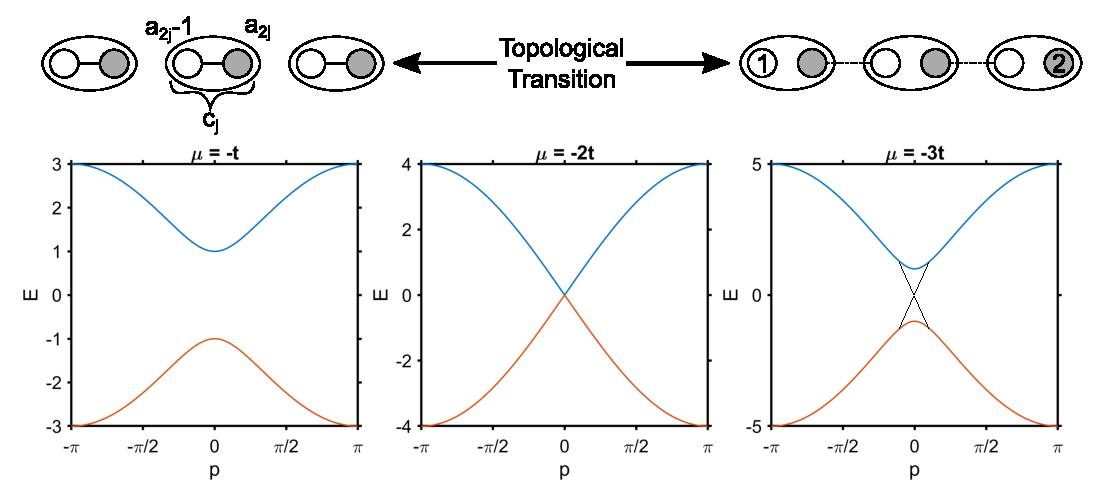
\includegraphics[width=\textwidth]{Intro/Figures/PWave_SC.eps}
	\caption{Dispersion relations of a 1D p-wave superconductor plotted at three different $\mu$ values. a) The trivial p-wave pairing scenario. The individual majorana particles each couple to the majorana on the same site. b) The critical value for $\mu$ where the gap closes. c) The topological p-wave pairing scenario. The majorana particles pair with majoranas on the nearest-neighbor site instead of on the same site. Two majorana zero modes are left on the edges of the wire, consistent with the bulk-boundary correspondence.}
	\label{pwavesc}
\end{figure}
For an intuitive picture for why this is we will split the complex fermion operators into their Majorana fermion constituents. We replace each complex fermion $c_{j}$ with two Majorana fermions, $a_{2j-1},a_{2j}$ via $c_{j}=\frac{1}{2}(a_{2j-1}+ia_{2j})$ and $c_{j}^{\dagger}=\frac{1}{2}(a_{2j-1}-ia_{2j})$. The Majorana operators are fermionic and are defined by their property $a_{j}=a_{j}^{\dagger}$ therefore they satisfy $\{a_{j}^{\dagger},a_{j'}\}=2\delta_{jj'}$ as well as $\{a_{j},a_{j'}\}=2\delta_{jj'}$. As an aside, due to the latter relation we can always break up a complex fermion operator into its real and imaginary Majorana components, although it may not always be a useful representation. Now, the Hamiltonian for the lattice p-wave superconductor can be written as:
\begin{align}
	H_{BdG} = \frac{i}{2}\sum_{p}\left(-\mu a_{2j-1}a_{2j}+(t+|\Delta|)a_{2j}a_{2j+1}+(-t+|\Delta|)a_{2j-1}a_{2j+2}\right)
\end{align}
Here we can examine the difference between the two cases presented above by looking at two special limits.\par 
The first limit is the trivial phase when we choose $\mu < 0$ and $|\Delta|=t=0$. Here, the Hamiltonian reduces to,
\begin{align}
	H = -\mu\frac{i}{2}\sum_{j}(a_{2j-1}a_{2j})
\end{align}
In this phase, the Majorana operators on each site are coupled together with an energy $\mu/2$ but there is no coupling between Majorana operators on different sites (see Fig \ref{pwavesc}). This is denoted as the trivial phase since there will be no low-energy states on the end of the chain if the boundaries are cut between sites. Said another way, the Majorana operators are localized to each site and are therefore in the atomic limit which is to say the trivial ground state.\par 
The second limit is the topological phase where we choose $|\Delta|=t>0$ and $\mu=0$. Here, the Hamiltonian reduces to,
\begin{align}
	H=it\sum_{j}a_{2j}a_{2j+1}
\end{align}
This phase is the opposite of the previous phase as the Majorana operators on each site are only coupled to Majorana operators on \textit{different} sites with an energy $t$. When the chain is cut the Majorana operators $a_{1}$ and $a_{2L}$ ($L$ is the last site) are ``unpaired" and therefore there is a low-energy state on the each end of the chain (see Fig \ref{pwavesc}). Comparing to before, it is impossible to adiabatically tune this phase back to the atomic limit and is thus a topologically non-trivial state.\par 


\chapter{Cleanroom-in-a-Glovebox}
\label{chap:chap2}
\todo{After writing proper intro, come back and make this flow.}
\section{\label{sec:level1}Introduction}
Fabrication of devices at the nano-scale is central to future efforts in exploring novel quantum phases of matter and building next-generation devices. Previously this was achieved by creating dedicated facilities where the entire space is filtered and dust minimized via special air handling and attire for all who enter. While these cleanrooms minimize the amount of dust and other particles that can damage mesoscale devices, they do not protect the samples from either oxygen or water, at the same time they require extremely expensive and energy-intensive investments. In contrast, gloveboxes provide an inert atmosphere for working with oxygen and water sensitive materials, with greatly reduced initial and operational cost.\cite{Chae2016} However, performing nanolithography in a glovebox risks contaminating the rest of the inert environment due to the various solvents involved. With these issues in mind, we've designed and constructed the cleanroom-in-a-glovebox to bridge the gap between these two approaches in order to prepare, fabricate, and characterize various scientific samples entirely within an inert argon atmosphere. The cleanroom-in-a-glovebox contains two separate work chambers where one chamber is devoted entirely to lithography and the other to preparation and characterization (Fig. \ref{fig:Overview}a). The system can be operated with minimal training, no need for special attire (i.e. gowning), and far fewer demands on the building. As such, the described cleanroom in a glovebox produces higher quality devices with air-sensitive materials, requiring far lower initial investment and operational cost than a traditional cleanroom. This makes the system described crucial in future efforts at training the quantum workforce and development of novel devices with a wider range of materials.

An overview of the system is shown in Fig. \ref{fig:Overview}a, with the lithography chamber, (discussed in the ``Fabrication'' section), containing a Heidelberg $\mu$PG101 Direct-Write system, an Angstrom NexDep Thermal Deposition and Plasma Etching system, and a Spin-Coating Systems G3 Spin Coater. The characterization chamber contains a WITec alpha300R confocal Raman system (Fig. \ref{fig:Overview}b \& Fig. \ref{fig:Characterization}b), a Nanomagnetics ezAFM (Fig. \ref{fig:Characterization}a), a home-built 2D material dry-transfer system, electronic BNC and banana cable feedthroughs. These two chambers are connected via a small antechamber which allows us to transfer samples into and out of the gloveboxes while also enabling simple transfer between boxes without contamination. Lastly, attached to the back of the glovebox is an intermediate chamber for attaching a vacuum suitcase (Fig. \ref{fig:Characterization}d). This allows receiving from and transferring to a wide array of UHV systems, providing compatibility with electron-beam systems, 
scanning tunneling microscopy (STM), molecular beam epitaxy (MBE), angle resolved photoemission spectroscopy (ARPES) and other cutting edge tools. As such our processes and design enable a range of scientific tools on nanoscale, air-sensitive materials, while simultaneously reducing the time, training and cost involved.    

\begin{figure}
    \centering
    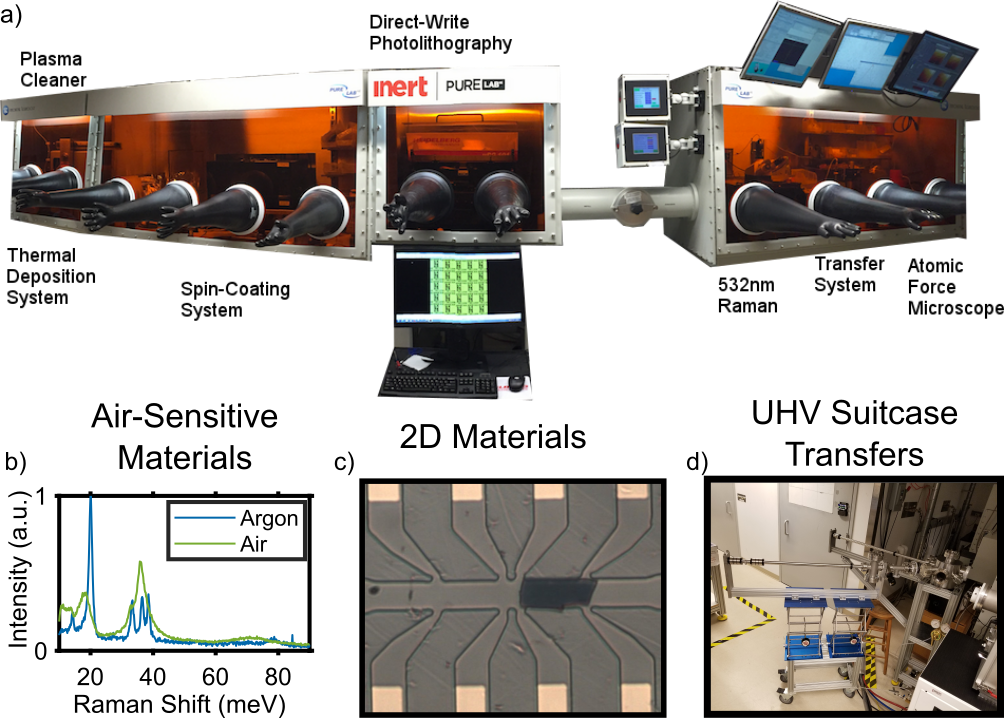
\includegraphics[width=\textwidth]{Chap2/Figures/IntroductionFigure.png}
    \caption{1a) Picture of the Cleanroom-in-a-Glovebox. b) Raman spectra measured on $\alpha$RuCl$_{3}$ showing the difference exfoliation in the inert atmosphere makes. Raman measurements were taken using the WITec Raman System installed in the glovebox. c) Bi$_{2}$Sr$_{2}$CaCu$_{2}$O$_{8+\delta}$ exfoliated onto a thin film of Ga$_{1-x}$Mn$_{x}$As. The film was then etched into a double hall-bar structure around the flake. d) Photo of the UHV suitcase during a device transfer from the glovebox to the low-temperature Raman system. The UHV suitcase is attached to the back of the glovebox.}
    \label{fig:Overview}
\end{figure}

\section{\label{sec:level2}Materials Characterization}
Atomic force microscopy (AFM) is an invaluable tool for characterizing materials. In the case of mesoscale physics, AFM is used to discern the thickness of exfoliated 2D materials. In other cases it characterizes the roughness of a substrate (such as in \ref{fig:Characterization}a) or sample. In order to resolve such small features, great care was taken to isolate the AFM system from environmental vibrations. This is more difficult than usual in a glovebox, as there are quite a few vibrations that arise from the gas-circulation system as well as sudden pressure changes from users inserting their hands into the glovebox to work on other tasks. To combat these vibrations the ezAFM and transfer stage were placed on a large granite slab. An additional Minus-K Vibration isolation stage was employed for the ezAFM and care was taken to ensure the cables were well secured to each other but did not touch the glovebox directly. The results of this are seen in Fig. \ref{fig:Characterization}a where we took an AFM scan of Mica, an atomically flat substrate. The noise levels of the scan are less than 5 angstroms in magnitude (the resolution of the ezAFM). To ensure rougher features can be resolved, this was compared with the AFM from HfO$_{2}$ film on a Si substrate grown by atomic-layer deposition. We note that ezAFM works with voice coils and thus is substantially less expensive and easier to use than a typical AFM system. Nonetheless, we anticipate a further reduction in noise with more traditional piezo-based scanning probes. 
\par
Raman spectroscopy can be used to tell the quality, doping level, thickness, symmetry, and cleanliness of samples.\cite{Ferrari:2013jx,Shahil:2010fg,Zhou2018,lei2019high,PhysRevB.82.064503,BTSAPLlocal2016} For example, the ratio of the 2D peak to the G peak in graphene is commonly used to discern how disordered the sample is.\cite{wu2018raman} With our Raman system's mapping capabilities, we determined the spatial distribution of the disorder after the fabrication of CVD graphene such as in Fig. \ref{fig:Characterization}b. The WITec system also allows us to measure photoluminescence (PL) with a simple switch of energy ranges. PL is a useful measurement technique when working with materials such as MoS$_{2}$, as it quickly identifies single-layer flakes, and provides insight into the interaction of MoS$_{2}$ with the substrate.\cite{YHlee2017review,yin2011single,Butler:2013ha} We observed another advantage of the glovebox here. Namely, Mica is known to have charged potassium ions on the surface after cleaving but is quickly neutralized in air.\cite{Lui2009} When exfoliating MoS$_{2}$ directly to the mica we found the PL consistent with the mica taking the MoS$_{2}$ from n-type to intrinsic.\cite{Mak2013,Ross2013} (see Fig. \ref{fig:Characterization}c) 

It is crucial to overcome the ``glovebox-specific'' problems to obtain the high-quality Raman and PL data. These are two-fold, first additional light contamination adding unwanted background signals and change in focus or position of the sample due to vibrations, air currents, and temperature fluctuations. To minimize these effects a simple casing was placed around the entire system, using black plastic sheets and 80-20 aluminum bars. Combined with careful isolation of the fibers and wires via foam sealing to the glovebox, the case enabled high-resolution Raman and PL area-scans like the one shown in Fig. \ref{fig:Characterization}b and c.
\begin{figure}
    \centering
    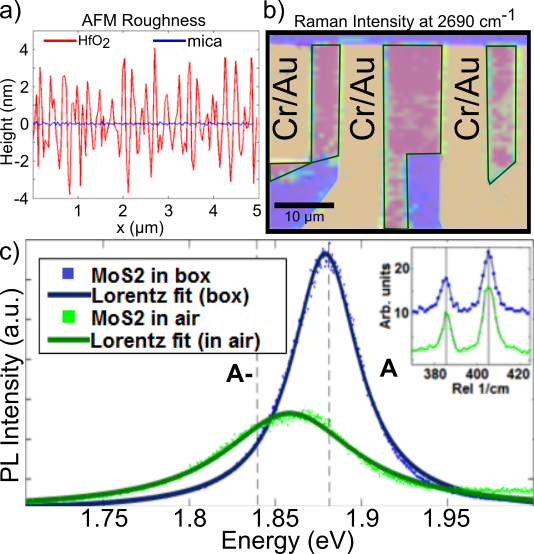
\includegraphics[width=88.9mm]{Chap2/Figures/CharacterizationFigure.png}
    \caption{a) Line scan using the \textit{in-situ} AFM on a halfnium oxide and mica substrate. This data demonstrates both the effectiveness of our vibration isolation methods and the atomically flat surface of mica. b) Area scan of a patterned CVD graphene device using the \textit{in-situ} Raman system. Graphene is outlined in green while color represents the intensity of the 2D-peak. c) Photoluminescence of MoS$_{2}$ exfoliated on mica. Blue data represents MoS$_{2}$ which was exfoliated onto mica in the glovebox while green represents exfoliation in the ambient environment. The inset shows Raman spectroscopy in the same conditions as the PL. We note that since the phonon modes do not shift in energy we can attribute this drastic change in PL to the inert glovebox environment and not to the dielectric characteristics of the substrate.}
    \label{fig:Characterization}
\end{figure}

\section{\label{sec:level3}Sample Fabrication}
The ability to create mesoscopic heterostructures has been crucial in the study of 2D materials, by enabling new physical effects and allowing encapsulation for removal to air.\cite{Dean:2012ht,Sharpe2019,Wu2018WTe2,stepanov2018long,Tang2017WTe2,Zareapour:2012ja,Island2019,Chae2016} However, this relies on minimizing additional contaminants from solvents. Thus we constructed a standard dry-transfer system in the characterization chamber. To ensure excellent alignment and minimal drift during transfer, the stage was placed on a thick granite slab, with the required wires and tubing isolated from touching the glovebox chamber directly. The transfer stage has six, fully-motorized stages, three of which are piezo-based Picomotor stages with a 30 nm step size providing precise positioning of the samples relative to one another, such as the heterostructure shown in Fig. \ref{fig:Overview}c. Furthermore, this system has produced a number of complex devices including the realization of Coulomb Blockade into atomic defects in a 2D heterostructure\cite{Brotons-Gisbert2019}, observation of hinge modes in a higher order topological superconductor,\cite{Gray2019} and CVD graphene sensors of bacteria with single cell resolution\cite{KUMAR2020112123}. 

One of the key features of our cleanroom in a glovebox is our photolithography capabilities. In our fabrication chamber, we have an SCS G3 Spin Coater, Angstrom Engineering NexDep physical vapor deposition system, a UHV suitcase transfer system, and a Heidelberg $\mu$PG101 Direct-Write system. The glovebox column has a solvent scrubber installed, which allows for small amounts of solvent to be removed from the system. This keeps the rest of the environment clean while using the photolithographic, lift-off, and cleaning solvents. We employ the use of Qorpak bottles to limit the exposure of solvents to the glovebox atmosphere. These bottles have a PTFE liner in the caps that are resistant to most chemicals while also providing a low moisture transmission rate. In addition, we use activated charcoal as a passive solvent absorbent. Raman, PL, and AFM scans of materials before and after long term exposure to the fabrication chamber revealed no evidence for additional contamination. This is further attested to by our ability to observe quantum oscillations at relatively low fields in graphene devices fabricated inside (Fig. \ref{fig:FabricationFigure}c). 

The lack of contamination along with the alignment abilities of the mask-less system was crucial in creating high-quality devices and periodic structures (see Fig. \ref{fig:FabricationFigure}d and \ref{fig:FabricationFigure}e). The $\mu$PG101 has a resolution of $1~\mu m$ with a $20~nm$ registry, optical auto-focus and can write up to a 5-inch wafer in one run. We note optical auto-focusing is required as the changing dynamics of the glovebox air prevented the use of standard pressure alignment. The $\mu$PG101 stage runs on an air-bearing that is normally supplied with compressed air from the building, but this is not possible while in a glovebox as the unfiltered air would vent directly into the clean environment. Instead, we inserted a T-junction into the argon path from the cylinder where one side of the junction goes into the cylinder to supply the glovebox and the other supplies the stage with argon for the air-bearing. Not only does this solve the air-bearing problem but it also vents excess solvents and water from the clean atmosphere more quickly. To shut off the air-bearing when the system is not in use, we installed a cutoff valve after the T-junction that is shut when the stages don't need to move.
\par

\begin{figure}
    \centering
    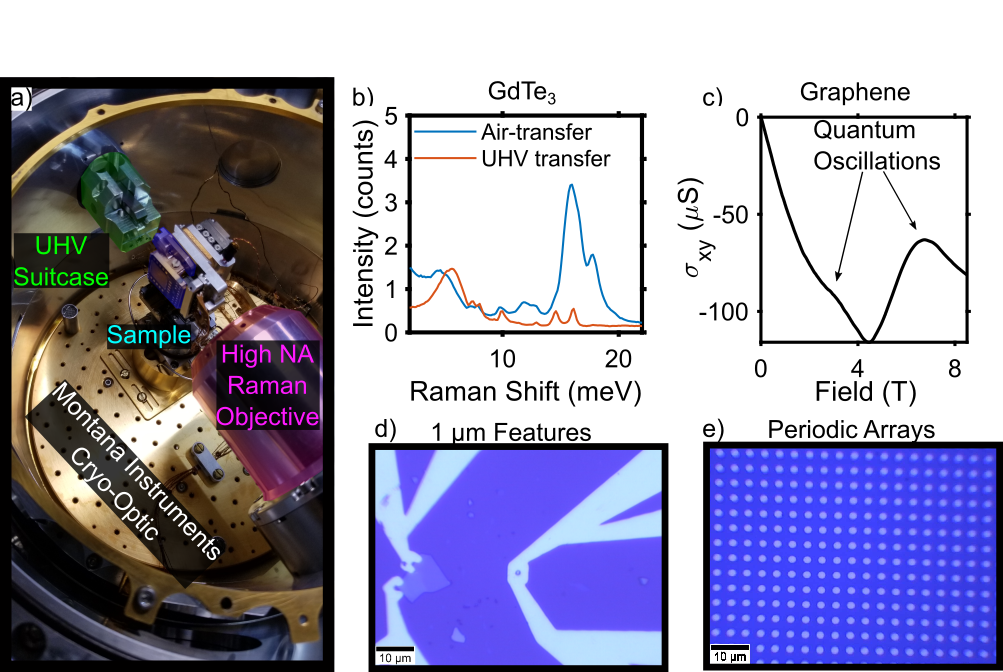
\includegraphics[width=\textwidth]{Chap2/Figures/FabricationFigure.png}
    \caption{a) Photo taken when transferring a sample from the glovebox into the Low-temperature Raman system. Highlighted in green is the transfer arm from the UHV suitcase, in blue is the sample holder mounted onto the cryocooler, and in purple is the high NA Raman objective. b) Comparison of Raman spectra of GdTe$_{3}$ demonstrating the degradation of the sample when exposed to air for even a few minutes. c) Hall conductance versus Magnetic Field for a CVD grown graphene sample, fabricated into a hall bar geometry in the glovebox. Even at 7 K, the sample shows quantum oscillations (see arrows). d) Superconducting aluminum loops of 1 $\mu$m radius fabricated onto FeTe$_{0.55}$Se$_{0.45}$ demonstrating the single micron resolution of the $\mu$PG101 photolithography system. e) Periodic arrays of 1 $\mu$m gold pillars.}
    \label{fig:FabricationFigure}
\end{figure}

In a typical nanofabrication process, one must develop and dry the samples in air before moving them into a deposition tool. With an \textit{in-situ} thermal deposition system glovebox users are able to develop and dry the sample in the inert argon environment before transferring them into the deposition tool. Furthermore, the deposition tool contains an \textit{in-situ} plasma-cleaning system so samples can be de-scummed in high vacuum immediately before the deposition of metals. This step can be critical in establishing good electrical contact to certain materials. Following the deposition, small amounts of aluminum can be evaporated onto the samples followed by exposure to a 0.1\% oxygen environment, creating an air-protection layer of alumina.\cite{Damasco2019tunnel} This layer of alumina can also be used to protect samples against photoresists during nanofabrication processes as it is easily removed by TMAH-based developers. For example, when fabricating CVD graphene devices we first deposit a layer of alumina before spin-coating photoresists while the rest of the fabrication process remains exactly the same, including energy dosage and developing times. The areas of photoresist that are developed out also allow for the developer to come in contact with the alumina, removing it as well. Thus we are still able to make good electrical contact to the graphene while preventing contact with the photoresist and other potential dopants.

The deposition tool also opens to the outside allowing users to clean samples with argon plasma or thermal annealing before loading them into the glovebox. An example is our fabrication of CVD graphene devices for use in bio-sensing applications. The CVD graphene is grown on copper foil and thus must be transferred onto SiO$_{2}$/Si wafers via wet transfer.\cite{doi:10.1021/acsnano.6b04110} In order to clean the graphene, we bake the samples in the deposition tool at 350 $^{o}$C in 10$^{-7}$ mBar pressure for nine hours before alumina deposition (described above) then subsequently transferring samples into the glovebox for patterning. The result of this is samples that are clean enough to not only see quantum oscillations at 8 K and 7 T shown in Fig. \ref{fig:FabricationFigure}c, but are also able to be used as single-bacterium bio-detectors.\cite{KUMAR2020112123}

\section{\label{sec:level4}Ultra High Vacuum Suitcase}
After fabrication, samples typically must be taken out of the glovebox to be measured in more specialized pieces of equipment such as surface-sensitive (STM, APRES) or low-temperature  transport and optical probes. Furthermore, many new materials and heterostructures are first created by MBE, requiring \textit{in-situ} probes to determine their device characteristics.\cite{Gerber2017FeSe,Wang2016,Hellman2017Rev} This presents a chance for the samples to see air and degrade. Typically this is avoided by coating the samples with a ``capping-layer'' (e.g. alumina) or covering mesoscale samples with hBN. However, samples may interact with these materials in unexpected ways such as accidental electrical shorting if the alumina contains many pinholes or if the hBN induces strain into the samples. The addition of hBN to an exfoliated flake could cause additional complexities including changing the dielectric environment or inducing Moire patterns that, while exciting, make reproducibility of devices quite difficult as both layers must be aligned in the same orientation for every device.\cite{Sharpe2019,Woods2014,doi:10.1021/nl5006542,Tran:2019aa,Jin:2019aa,Alexeev:2019aa,Yankowitz2019,Cao2018} Another exciting example of eliminating hBN from air-sensitive devices is the $\beta$-Fe$_{1.1}$Se crystal, where recent experiments have shown enhancements of T$_{c}$ in monolayer films as compared to bulk samples but clean monolayer-devices have yet to be realized.\cite{Gerber2017FeSe,Wang2016} This is in part due to the air-sensitivity of the system at low layer numbers but is also due to the crystal's sensitivity to strain.\cite{Yang2019} Recent experiments have shown that the T$_{c}$ of $\beta$-Fe$_{1.1}$Se thin films change as much as 10 K with 1\% strain which demonstrates the problem in making hBN encapsulated devices.\cite{Kawai2018} 

To expand the range of probes and fabrication capabilities of the cleanroom-in-a-glovebox, we designed and built a UHV chamber to couple to various vacuum suitcases (see Fig. \ref{fig:Overview}d). The intermediate chamber has a block for attaching different kinds of sample holders allowing us to transfer materials into the glovebox from MBE and out to STM, low-temperature Raman, or electrical transport systems (e.g. see Fig. \ref{fig:FabricationFigure}a). One measurement system of particular interest is the custom-designed Montana Instruments low-temperature Raman system. This system has been described in detail in other works\cite{Tian2016} but has been adapted to be compatible with a UHV suitcase. All of the suitcases that are used follow typical transfer procedures with the addition of a connection to an inlet for Argon gas. Specifically, after the sample is brought into the intermediate space, the suitcase is valved off and Ar added to bring the chamber to match the glovebox pressure. Once matched the intermediate chamber is opened to the glovebox, where the sample holder is brought in using a second manipulator arm. When transferring devices out of the glovebox a baking step is added to the normal process after vacuuming where the entire chamber is heated to 120$^{o}$C. This step helps remove any excess impurities introduced when exposing the intermediate chamber to the glovebox.

The merits of such work are shown in Fig. \ref{fig:FabricationFigure}b, where we probe the Raman response of GdTe$_{3}$, established to be highly air sensitive.\cite{lei2019high} Two bulk crystals were prepared in the glovebox, then one was transferred into the low-temperature Raman system in air and freshly cleaved just before cool down. The second sample was transferred via the UHV suitcase. The crystal that was transferred in air clearly shows a large tellurium oxide peak around 17 meV that obscures phonon modes.\cite{YaoCGT2Dmat,lei2019high} However, the material transferred via vacuum suitcase revealed sharp phonon modes, with the exception of the CDW amplitude mode at low energies. In addition, we found the Raman response to be much more uniform across the sample surface. 

\section{Conclusions}
Here we demonstrated the construction and operation of a cleanroom-in-a-glovebox. The system combines the inert environment of a glovebox with the fabrication and characterization facilities of a cleanroom. While modifications had to be made to existing equipment and procedures, the result is a fast and efficient fabrication facility that allows devices made from many air-sensitive systems that were previously unattainable. In addition, the far reduced cost, ease of use, and environmental requirements open the door to using this setup in a wider array of educational as well as research settings.  
 
\chapter{Topology in FeTe\texorpdfstring{$_{0.55}$}{0.55}Se\texorpdfstring{$_{0.45}$}{0.45}}
\label{chap:CRAIG}
\todo{After edits to Chapter 2, come back and make this flow.}
\section{Introduction}
New particles can be a convincing signature of emergent phases of matter, from spinons in quantum spin liquids\cite{Balents2010} to the Fermi arcs of Weyl semimetals\cite{Armitage2017,Zhang2019}. Beyond potentially indicating a broken symmetry or topological invariant, they can be put to use in future topological quantum computers\cite{Nayak2008}. Until recently it was believed the non-trivial topology of the bulk would lead to new states in one lower dimension at the boundary with a system of differing topology. However, higher order topological insulators (HOTI) have been realized\cite{Schindler2018,Ni2018,Xue2019,Song2017,Langbehn2017,Benalcazar2017}, where the resulting boundary modes exist only at the intersection of two or more edges, producing 1D hinge or 0D bound states. One route to creating these higher order states is through the combination of a topological insulator and a superconductor with anisotropic pairing\cite{Wang2018Corner,DasSarma2018,Zhongbo2018,Ghorashi2019}. Usually, this is done by combining two separate materials and inducing superconductivity into the TI via proximity\cite{Zareapour2012,Albrecht2016,Gazibegovic2017,Kurter2018,Tanaka2012}. However, this method requires long coherence lengths and extremely clean interfaces, making experimental realization of devices quite difficult. For studying HOTI, as well as the combination of strong correlations and topology, the material FeTe$_{0.55}$Se$_{0.45}$ (FTS) may be ideal, as it is a bulk, high-temperature superconductor with anisotropic pairing that also hosts topologically non-trivial surface states\cite{Zhang2018,Wang2015,Wang2018}.
\begin{figure}
    \centering
    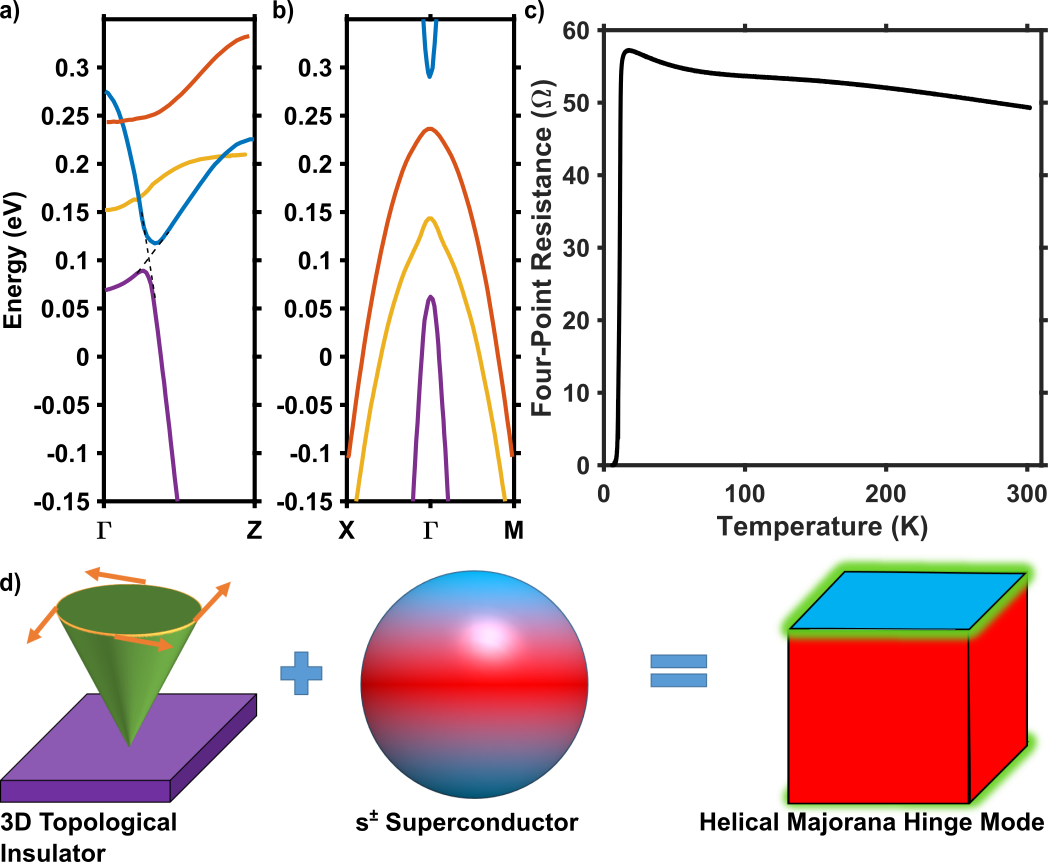
\includegraphics[width=\textwidth]{Chap3/Figures/F1V1.png}
    \caption{a) Theoretical band structure of FeTe$_{0.55}$Se$_{0.45}$ along the $\Gamma$-Z and (b) the X-$\Gamma$-M cuts\cite{Wang2015}. The $p_{z}$ orbital of the chalcogenide is shown in blue, crossing the three d-orbitals, resulting in two Dirac points and topological, spin-orbit gap. c) Resistance vs. Temperature graph for an exfoliated flake of FTS, showing a clear superconducting transition around 10K. d) Diagram showing the ingredients needed for a Helical Majorana Hinge Mode}
    \label{HingeTheory}
\end{figure}



\par
FTS is part of the FeTe$_{1-x}$Se$_{x}$ family of Fe-based superconductors, which ranges from an antiferromagnet in FeTe to a bulk superconductor in FeSe\cite{Liu2010}. These generally have the same Fermiology as the other Fe-based superconductors in that there are hole pockets at the $\Gamma$-point and electron pockets at the M-points\cite{Homes2015,Hanaguri2010,Miao2012,Okazaki2012,Zhang2018}. The relative strengths of the interband vs intraband scattering in principle should determine the superconducting symmetry, however, there is a complex interplay between the spin-fluctuation exchange, intraband Coulomb repulsion, and the doping level that all contribute to the symmetry of the superconducting order parameter\cite{Kreisel2016,Chubukov2012}. Indeed, experiments performed on FeTe$_{0.55}$Se$_{0.45}$ find no evidence for a node with strong signatures of s$^{\pm}$ order,\cite{Hanaguri2010,Miao2012,Zeng2010} while experiments on other alloys suggest nodal s$^{\pm}$, anisotropic s-wave, and even p-wave\cite{Michioka2010,Serafin2010,Bendele2010,Kim2010,Okazaki2012}. Interestingly, tuning away from FeSe leads to enhanced spin-orbit coupling and bandwidth. As a result, the p-orbital is shifted down in energy, crossing the d-orbitals with opposite parity along the $\Gamma$ to $Z$ direction (See Figure \ref{HingeTheory}a and b). The first two crossings are protected by crystalline-symmetry resulting in bulk Dirac states above the Fermi energy. However, the lowest energy crossing is avoided resulting in a spin-orbit coupled gap, resembling those typically found in topological insulators\cite{Wang2015,Chen178}. While the Fermi level falls into this gap, the original hole and electron Fermi surfaces at $\Gamma$ and $M$, respectively, are retained\cite{Zhang2018,Wang2015}. ARPES measurements have observed the resulting spin-momentum locked surface states, as well as their gaping out in the superconducting state\cite{Zhang2018,Zhang20192}. Additionally, there is evidence from STM that this results in apparent Majorana zero-modes inside magnetic vortices\cite{Wang2018,Dong-LaiFeng2018,Machida2018}.
\par
Recent theoretical work on FTS has suggested that the combination of an s$^{\pm}$ order parameter and topological surface states could give rise to higher order topological superconductivity\cite{DasSarma2018}. In short, the changing superconducting phase causes the surface states to gap out anisotropically. Depending on the relative strength of the isotropic versus the anisotropic term, this could lead to the [001] and the [100] or [010] face having superconducting order parameters with opposite phase. As shown in Figure \ref{HingeTheory}d), this is predicted to produce a pair of 1D Helical Majorana Hinge Modes emerging at the 1D interface of the top/side surfaces\cite{DasSarma2018}. Whether or not the modes we observe are indeed Majorana modes, the appearance of HHZM requires both s$^{\pm}$ superconductivity as well as strong 3D TI surface states. Thus observing Helical Hinge Zero Modes in FTS would provide strong evidence that it is an s$^{\pm}$ topological superconductor.
\par
To search for the HHZM it is tempting to rely on methods previously exploited to reveal the unconventional nature of the cuprates\cite{Deutscher2005}. Specifically, normal-metal/superconductor junctions demonstrated Andreev Bound States resulting from the d-wave order only on [110] surfaces\cite{Tanaka2003,Sinha1998,Greene1999,Tanaka2012}. In the case of FTS, this approach is more challenging as one must tunnel into the hinge between [001] and [010] and the modes are nominally charge neutral, thus requiring an Andreev process to be observed\cite{zhang2017quantum}.  To achieve this, we created 2D atomic crystal heterostructures with thick hBN covering half of the FTS. By draping contacts over the side of the FTS or atop the hBN we can separately probe conductance into the hinge from the c-axis. As expected for modes protected from back-scattering, we find a cusp-like zero-bias peak only on the hinge contacts that is absent from the c-axis junctions. The mode is well-described by a Lorentzian, consistent with other studies on one-dimensional zero-energy bound states\cite{Setiawan2017}. Confirmation that the mode does not result from our fabrication method or defect density is provided by soft-point contact measurements on facets of various bulk crystals (See Supplemental Fig S3). Taken together these data strongly suggest the presence of the HHZM in FTS resulting from its higher order topological nature and the presence of s$^{\pm}$ superconductivity\cite{Park:2010wo,Tanaka2012}. 
The helical hinge zero mode in FTS should only exist in the superconducting state. As such we expect a sharp zero-bias conductance feature below T$_{c}$ on the hinges between the [001] and side surfaces as compared to purely on the [001] face. Alternatively, Majorana zero modes on the hinge should give quantized conductance, revealed through nearly perfect Andreev reflection.\cite{DasSarma2018} However, as discussed later, observing this quantized conductance may be challenging as the coherence length in FTS is $\approx 3 nm$\cite{Kim2010,Bendele2010}. To test this we used 2D atomic crystal heterostructures to simultaneously fabricate Normal Metal/Superconductor (NS) low-barrier junctions on various crystal facets (See Figure \ref{MainResults}a and \ref{MainResults}d). The first type of NS junction is a standard lithographically-defined contact that drapes over the edge of the exfoliated flake. This contact will form a junction with the [001] and [100] surfaces as well as the hinge between them. The second type of contact is fabricated by first transferring hexagonal Boron Nitride (hBN) over half of the FTS flake, insulating the side and edge from electrical contact. We then drape a contact over the side of the hBN, forming a junction primarily on the [001] face (See depiction of the side view in Fig \ref{MainResults}d). The entire fabrication process, from exfoliation to device, is performed in an inert argon atmosphere or vacuum. Patterns for mesoscale contacts were defined using standard photolithography techniques and our Heidelberg $\mu$PG101 direct-write lithography system. Contact areas are then cleaned with an argon plasma at high vacuum immediately before thermal deposition of 5nm of Cr then 45nm of Au. Full fabrication details can be found in the Supplementary.
\par
\begin{figure}
    \centering
    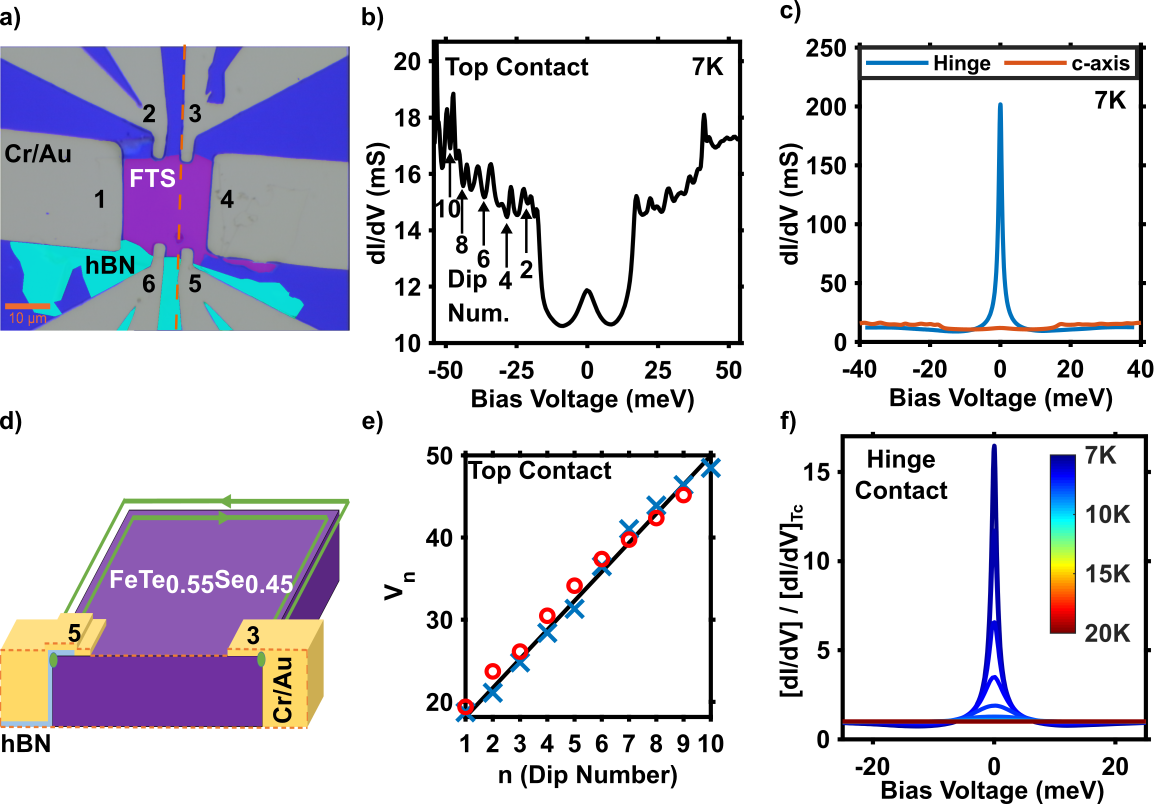
\includegraphics[width=\textwidth]{Chap3/Figures/Figure2.png}
    \caption{a) False color image of the exfoliated device; numbers denote contacts used. b) $\frac{dI}{dV}$ vs DC Bias voltage for contact 5 at 7 K. c)$\frac{dI}{dV}$ vs DC Bias voltage for contact 3 at 7 K. d) Depiction of contact geometry for top only (5) and hinge (3) contacts. e) Dip number vs. Voltage for c-axis only contacts. The black line is a fit to McMillan-Rowell Oscillations which follow the equation, $\Delta V = n\times\frac{hv_{F}}{4ed_{s}}$. Blue and red points are experimental data extracted from the positive and negative bias voltages respectively. f) Temperature dependence of differential conductance for various temperatures.}
    \label{MainResults}
\end{figure}
\section{Results and Discussion}
We first established that our control contacts are only tunneling into the c-axis by studying their base temperature differential conductance. Specifically, we sourced current between a top contact (5 or 6 in Fig. \ref{MainResults}a) to one of the current leads (\#1 or \#4), while measuring the resulting voltage between the same top contact and the other current contact. This three-point experiment ensures the conductance results primarily from the interface of the top contact. As shown in Fig \ref{MainResults}b, we observe a small zero bias conductance peak that is $\approx 20 \%$ higher than the background. The shape and height are consistent with previous point contact Andreev reflection measurements along the c-axis of FeTe$_{0.55}$Se$_{0.45}$,\cite{Daghero2014} and confirms the contacts are in the low-bias, Andreev regime. We note these previous works were performed at temperatures below our base temperature, and as such could resolve the rather small gap. At higher bias, we observe an enhancement in the conductance  at $|V|\geq 20~meV$, consistent with spin-orbit induced gap. Above this value, we observe a series of conductance dips that are fully consistent with McMillan-Rowell Oscillations (MRO)\cite{2004PhyC..408..618C,2004PhRvB..69m2507S}. These MRO result from Fabry-Perot like interference of quasiparticles in the normal layer undergoing AR at the interface and reflecting off the back surface of the metal. The MRO are linearly spaced by voltages\cite{2004PhyC..408..618C} defined by the equation $\Delta(V) = n\cdot\frac{ev_{F}}{hd}$ where n is the dip number, $v_{F}$ is the Fermi velocity at the contact, and $d$ is the thickness of the metal which we set to 50~nm (See Figure 2e). From this fit, we extract a renormalized Fermi velocity of approximately $1.7\times10^5 m/s$.  We note that similar behavior was observed if the current/Voltage was reversed between contacts \#1 \& \#4, we measure from contact \#6, or measuring between contacts \#6 and \#5 exclusively (see Supplemental Fig S4a). This shows the robustness of these results and combined with the detailed spectra, confirm the contacts over the hBN are Andreev tunneling only into the c-axis. 

Next, we turn to the spectra measured in an identical manner, but with the hinge contact (\#3 in Fig. \ref{MainResults}a). Since the normal-state and high bias resistance of the hinge contact is nearly identical to the control contact we expect the spectra to be similar. However, as shown in Fig. \ref{MainResults}c the zero-bias conductance in the hinge contact is quite distinct from the response observed in the control contact and previous point contact experiments. Specifically, we observe a cusp-like zero-bias conductance peak (ZBCP) in the hinge contact that reaches a value 17-times higher than the high bias or $T\approx T_{c}$ conductance. This rather large enhancement is also likely responsible for the absence of a clear observation of the gap, which would be far smaller. These results provide strong evidence for a zero mode that only exists on the hinge. The "cusp-like" shape and magnitude of the peak could result from an Andreev Bound State (ABS)\cite{Deutscher2005,Sinha1998,Greene1999}, however, this requires either a node in the superconducting gap or time-reversal symmetry breaking,\cite{Yakovenko2002,TanakaTopSym2012} neither of which has been detected in FeTe$_{0.55}$Se$_{0.45}$\cite{Serafin2010,Zeng2010,Bendele2010,Okazaki2012,Miao2012,Kim2010,Hanaguri2010}. As discussed later, direct evidence against the ABS interpretation is provided by the dependence of the peak on temperature, and near independence on the contact's type (planar, point contact) or material (Ag, Au, Bi$_{2}$Te$_{2}$Se$_{1}$). Interestingly, this behavior is also inconsistent with previous observations of standard Andreev Reflection(AR)\cite{Tanaka2003}, Coherent Andreev Reflection (CAR)\cite{Klapwijk1992}, the Kondo Effect\cite{Sasaki2000,Samokhin2001}, and Joule heating\cite{Naidyuk2018}. 

To ensure the zero bias conductance peak emerges at T$_{c}$ and is not the result of an ABS, we directly analyzed its temperature dependence by fitting the data with a Lorentzian line shape. This is based on recent theoretical studies on one-dimensional superconducting wires showing that both Majorana Zero Modes and ABS produce a Lorentzian differential conductance spectra\cite{Setiawan2017}. While this may not be the correct model for our case, to the best of our knowledge there are no calculations for the conductance spectra expected from hinge modes in a higher order topological superconductor. Nonetheless, the differential conductance spectra are generally well described by a Lorentzian (see Fig \ref{DataAnalysis}a). The temperature dependence of the height and width of the peak determined by the fits for the data presented in Fig. \ref{MainResults}f are shown in Fig. \ref{DataAnalysis}b \& c, respectively. These data provide direct evidence for the connection to the bulk superconductivity, though are inconsistent with an ABS. Indeed, we find that as the temperature is raised, the height of the ZBCP decreases exponentially until it is completely quenched at $T_{c}$ (see Fig\ref{MainResults}a and Fig\ref{DataAnalysis}b), where we define $T_{C}$ as the temperature for which $\frac{dR}{dT}$ passes through zero. While lower temperature data are required to determine the exact functional form, it is clear from Fig. \ref{DataAnalysis}b \& c that the mode is substantially different from the $1/T$ behavior typically expected from an ABS. Furthermore, we found a similar shape and temperature dependence in contacts of various barrier height, also inconsistent with standard Andreev reflection.\cite{BTK,Tanaka2012,Lofwander2001}

Similar to the height of the peak, we find the width of the zero bias conductance peak grows exponentially with temperature (see Fig. \ref{DataAnalysis}). Interestingly the energy scale governing the peak height ($E_{H}\approx 0.08~meV$) and the width ($E_{\Gamma}\approx 0.1~meV$) are quite close. We note that comparable results were obtained from other contacts revealing the hinge mode. Nonetheless, the energy scales governing the temperature dependence of the mode are far smaller than either the superconducting gap of the bulk or the surface states.\cite{Zhang2018} However, to the best of our knowledge, the size of the superconducting gap on the side surface has not been measured. As such we speculate this small apparent energy scale results from a much weaker proximity effect on the [010] and [100] surface states. Interestingly, extrapolating the width of the zero bias peak to zero temperature suggests an extremely narrow mode ($\approx 3.5~\mu eV$). While further studies at lower temperatures are required to confirm this extrapolation and the specific shape of the mode, if correct it points to the highly coherent nature of the excitation. As such the temperature dependence is consistent with our expectations for topologically protected 1D modes. 
\par
\begin{figure}
    \centering
    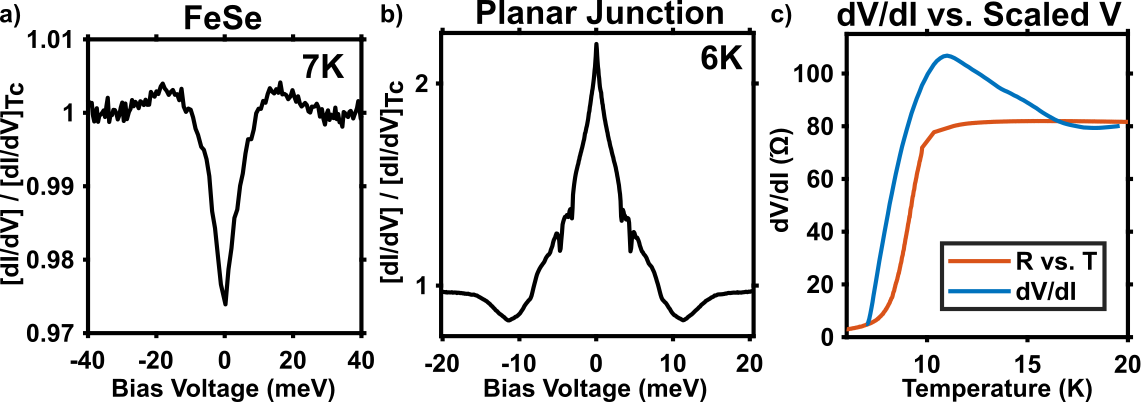
\includegraphics[width=\textwidth]{Chap3/Figures/Figure3.png}
    \caption{a) dI/dV versus voltage normalized to the spectra taken at T$_{c}$ (solid line) with a Lorentzian fit (dashed line), for $T=7K$, $9K$, and $15K$. b) and c) ZBCP heights and widths, respectively, extracted from the Lorentzian fit versus temperature. The exponential temperature dependence (orange lines) is at odds with a normal Andreev bound state that follows a $1/T$ dependence. The small energy scale of the exponential may result from the reduced superconducting gap on the side surfaces. While the rather small width at zero temperature is consistent with a topologically protected 1D mode.}
    \label{DataAnalysis}
\end{figure}
For additional confirmation that the ZBCP does not result from fabrication, exfoliation, impurities or the specific metal used in the contact, we performed a series of additional control experiments, summarized in Fig (\ref{Controls}). First, the topological gap in FTS closes with reduced tellurium levels, thus we expect the hinge mode is absent from FeSe. To confirm this as well as the irrelevance of contact type or normal metal used, we employed soft-point contact measurements. For FeSe we observe no evidence of an increase in conductance at zero bias below T$_{c}$ (see Fig (\ref{Controls}a). However, performing the same soft-point contact spectroscopy across multiple different FeTe$_{0.55}$Se$_{0.45}$ crystals always produces an increase in conductance at zero-bias when cooled below T$_{c}$ consistent with the data on contacts made via photolithography (see Supplemental Fig S3). The soft-point contacts revealed a smaller enhancement of the zero bias conductance in the superconducting state. However this is expected since the quasi-particle lifetime in the Ag paint contact is likely lower, which smears the spectra and reduces the height at zero bias. Similarly, we used planar junctions with Bi$_{2}$Te$_{2}$Se$_{1}$ via a method that has previously enabled spectroscopic studies with low barriers in van der Waals materials.\cite{Zareapour2012} As shown in Fig. \ref{Controls}b, these junctions also resulted in nearly identical spectra near zero bias. Here the lower zero bias conductance is expected as it contains contributions from the normal material being in series with the contact. Another extrinsic explanation for the peak is the interstitial Fe-atoms known to be present in these materials. However, we excluded this explanation by measurements on annealed samples where the Fe impurity content is dramatically reduced (see Supplemental Fig S3a), though the topology and Tc are only mildly affected.

An alternate mechanism for producing a ZBCP is Joule heating at the contact. We took a number of steps to rule this out. First, similar results were obtained regardless of the exact contact configuration (e.g. swapping contacts employed for current versus voltage in point contact or three-point measurements). In addition, we compared the voltage and temperature data by inverting the $\frac{dI}{dV}$ spectra and comparing it to the resistance versus temperature data taken on the same contact configuration (see Fig \ref{Controls}c). To align the two curves, we translate the $\frac{dV}{dI}$ curve such that zero voltage coincides with the temperature at which it was recorded (7 K). Next, we assume the voltage where the maximum resistance is measured is equivalent to heating to T$_{C}$, as this is the temperature where a peak in resistance is typically observed (see Fig \ref{HingeTheory}d). While the exact voltage dependence due to heating could be more complex, it is clear the $\frac{dV}{dI}$ versus voltage spectra are far in excess of the resistance measured at T$_{c}$, though at high bias they do return to the value measured at T$_{c}$. This further excludes voltage induced heating as the origin of the zero bias conductance peak. In addition, the background conductances in the c-axis, hinge, and point contacts are nearly identical. Therefore the heating across all of them should be approximately the same. However, they reveal quite distinct spectra (i.e. strong ZBCP in the hinge contact vs. nearly none in the c-axis) which, combined with the emergence of the zero-bias conductance peak (ZBCP) at T$_{c}$ in numerous contacts (see Figure \ref{MainResults} and Supplemental Figure S2), eliminates heating.
\par
\begin{figure}[H]
    \centering
    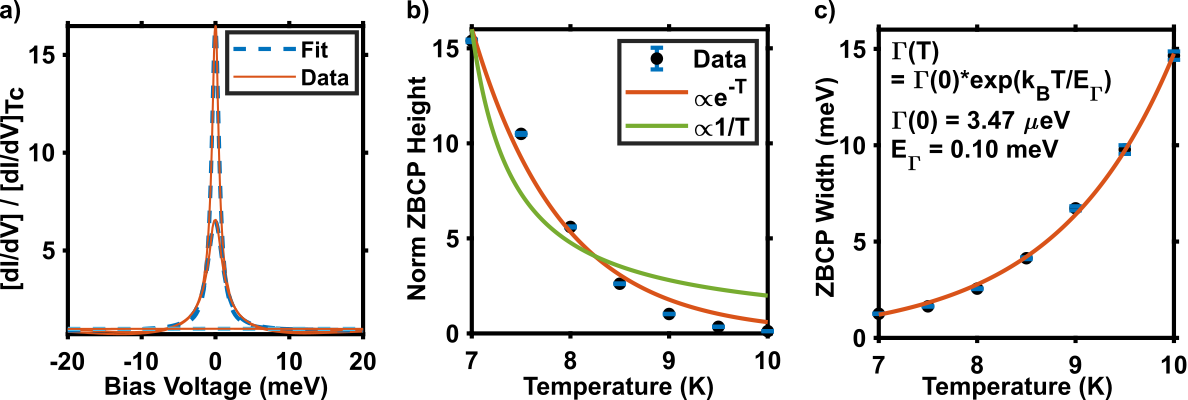
\includegraphics[width=\textwidth]{Chap3/Figures/Figure4.png}
    \caption{a) Soft-point contact on a bulk crystal of FeSe normalized to the critical temperature. b) Differential conductance using a planar junction, revealing a similar zero-bias peak. The smaller height results from the normal resistance of the Bi$_{2}$Te$_{2}$Se$_{1}$ that is in series with the tunnel contact. c) Differential resistance versus scaled voltage (blue) plotted along with the resistance versus temperature curve(orange). The strong overshoot of the voltage-dependent resistance and its return at high-bias to the normal state resistance confirms the spectra and zero bias conductance peak are not a result of heating.}
    \label{Controls}
\end{figure}
In summary, via a variety of contact methods, we reveal helical hinge zero modes in the topological superconductor FeTe$_{0.55}$Se$_{0.45}$. Specifically,  contacts to the [001] surface made using hBN reveal standard Andreev reflection, while those draped over the hinge contain a cusp-like, zero-energy feature in the differential conductance. By combining with measurements using soft-point contacts on various crystals, we further confirm the intrinsic nature of this new mode. Furthermore, the appearance of an HHZM in FTS helps to establish both the topological and s$^{\pm}$ nature of the superconductivity. An important question raised by these results is the large size and the temperature dependence of the HHZM. It is possible that the large ratio of contact area to coherence length at the measured temperature ($\approx 1000x$), makes the measurement essentially many point-like contacts in parallel, leading to an apparently large conductance. The contact size may also play a role in the temperature dependence, as could the unknown size of the superconducting gap on the side surface. Thus future theoretical and experimental efforts must be made to better separate out the contact effects from the intrinsic response of the hinge mode we observe. 
 
\chapter{New Results in FeTe\texorpdfstring{$_{0.55}$}{0.55}Se\texorpdfstring{$_{0.45}$}{0.45}}
\label{chap:PAR}
\section{Introduction}
Recent works have called into question the exact topological nature of \ac{FTS} claiming the crystal is not a topological insulator but rather a topological semi-metal with buried Dirac nodes. In light of this it is crucial to obtain evidence with more experimental techniques to better understand the nature of the topology in the \ac{FTS} system. Indeed, the underlying physics which predicts the helical hinge mode also predicts the same mode to manifest as a bias-independent conductance plateau in a differential conductance measurement rather than the previously observed zero-bias conductance peak. To accomplish this, we investigate the effect edge quality has on the topological characteristics of \ac{FTS} as it has been previously shown that the quality of the crystal edge can have a drastic effect on its transport characteristics \todo{cite Andrea's work on different transport characteristics of graphene}. We find that when tunneling measurements are performed across pristine, high-symmetry crystalline edges bias-independent conductance plateaus are observed for biases below the superconducting gap energy while ``rough" edges do not exhibit such plateaus. Furthermore, these plateaus are consistent with \acl{PAR}.

\section{Observation of Bias-Independent Conductance Plateau}
The tunneling conductance of a normal-metal/superconductor interface can be modeled by assuming an delta-function potential barrier at the interface characterized by a strength parameter $Z$, i.e., the \ac{BTK} method. An in-depth discussion and pseudo code for performing these simulations can be found in \ref{app:ARfit}], however we will take some of the main results of these calculations for discussions here. The \ac{BTK} method on a standard \ac{BCS} s-wave superconductor predicts a bias-independent conductance plateau only when the strength of the potential barrier between the normal-metal and superconductor is exactly zero. Even slight deviations from a zero-strength barrier result in significant dips around zero-bias, thus observing \ac{PAR} is exceedingly rare and typically only occurs only in extremely clean materials \todo{cite klein paper}. Therefore when \ac{PAR} is observed in a system it is usually due to an underlying mechanism which causes the incoming carriers to ignore the barrier completely; these mechanisms include forbidden backscattering due to topological spin-momentum locked bands and majorana zero-mode assisted tunneling, among others. \ac{PAR} has three unique identifiers in a differential conductance spectrum: a perfectly flat plateau, the plateau is at twice the conductance of the normal state, and the plateau extends out to the superconducting energy gap.\par
\begin{figure}[h]
    \centering
    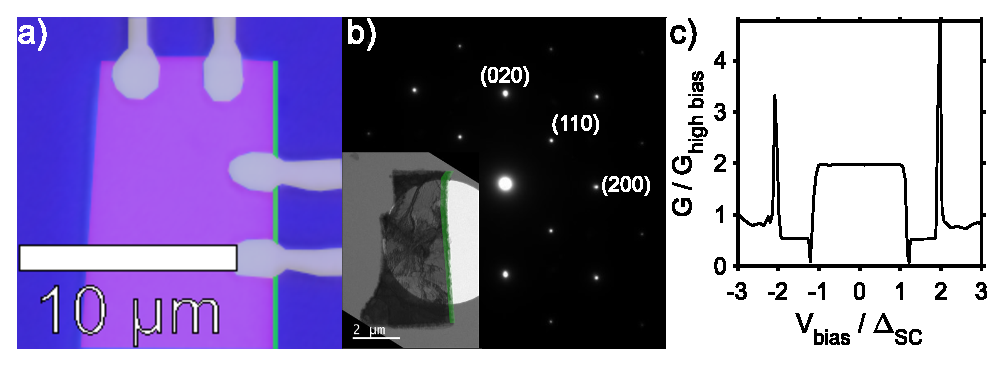
\includegraphics[width = \textwidth]{Chap4/Figures/DeviceFab.eps}
    \caption{a) False color optical image of a representative device with a straight (100) edge. b) \ac{TEM} diffraction pattern demonstrating the (100) edge. Inset shows the flake measured as well as the diffraction aperture. c) Base temperature differential conductance curve.}
    \label{fig:PARDeviceFab}
\end{figure}
\todo{Make Edge vs Plateau figure}
This bias-independent conductance plateau is observed in other devices with straight edges, however when performing tunneling experiments on ``rough" edges (i.e. edges that are not straight) the differential conductance does not show a plateau at low-biases (Fig \todo{fig ref}). This suggests that either the \ac{PAR} in this system is sensitive to the local contact conditions or the contact to the bulk superconductivity is greatly increased with rough contacts. In the first case, the topological nature of \ac{FTS} would be immediately called into question as the topology should not be affected by local crystal symmetry breaking. Indeed, this would seem to indicate that \ac{FTS} would be something closer to a Topological Crystalline Insulator. In the latter case, the \ac{PAR} is not affected by the local contact conditions but the signal is drowned out among a much larger supercurrent when better contact is made to the superconducting bulk.\par
\begin{figure}[h]
    \centering
    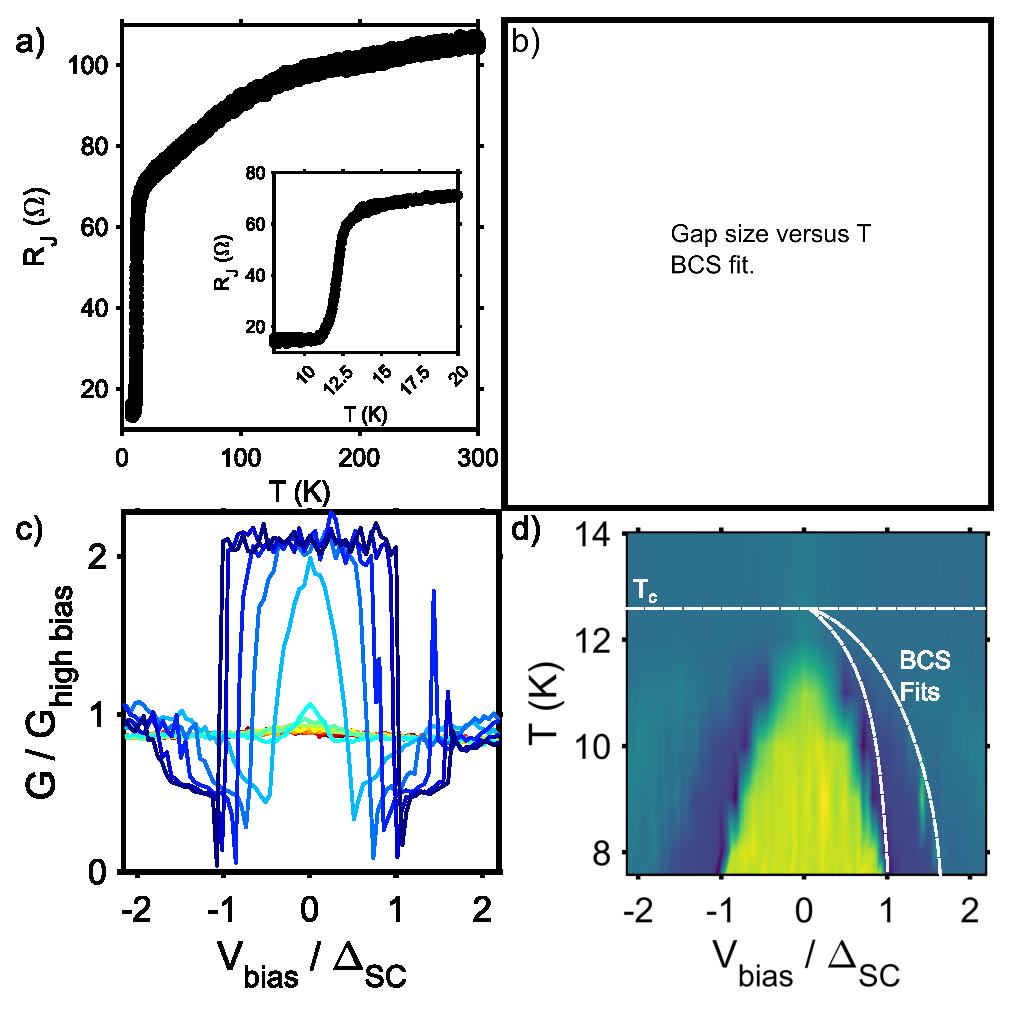
\includegraphics[width = \textwidth]{Chap4/Figures/Temperature.eps}
    \caption{Caption}
    \label{fig:PARTemp}
\end{figure}
While the temperature dependence of the width of this \ac{PAR} follows the \ac{BCS} model quite well, there is a striking difference when comparing the conductance at zero-bias to the \ac{BTK} model. Indeed, while a \ac{BTK} calculation with $Z=0$ displays a zero-bias conductance saturating around $T=0.1T_{c}$ the measured zero-bias conductance in \ac{FTS} saturates at a far higher temperature around $T = 0.9T_{c}$. This provides further evidence that the \ac{PAR} is not simply caused by lucky, perfect contacts as it seems the mechanism is only limited by the magnitude of the superconducting gap not by temperature.  

\section{Magnetic Field Dependence}
The Dirac surfaces states that are a key signature of a topological bulk are protected via time-reversal symmetry. It follows that if time-reversal symmetry is lifted via a magnetic field, any Dirac nodes that are aligned (the plane perpendicular to the spin-momentum locking determines the ``direction" of the cone) along the magnetic field will lose their topological protection. In contrast, if the Dirac node is perpendicular to the magnetic field, the node will simply shift up or down in energy but the node will keep its topological protection. In this manner, if the \ac{PAR} is caused by forbidden backscattering due to topological bands we expect highly anisotropic responses to different directions of applied magnetic field. While this seems to be the case in \ac{FTS} (shown in Fig \ref{fig:PARField}) we must be careful to differentiate the response of the \ac{PAR} from that of the bulk superconductor. Even though the upper critical field of \ac{FTS} is around $35 T$ \todo{cite field work} the bulk superconducting response of \ac{FTS} flakes is quite anisotropic, even below $9 T$ \cite{zalic2019}. When applying a magnetic field parallel with the hinge being measured (the a-axis of the material), the \ac{PAR} remains completely unaffected up to $5 T$. However, when the field is rotated to the c-axis of the crystal the \ac{PAR} seems to collapse quite rapidly which would give credence to a topological origin as discussed earlier. 
\begin{figure}[h]
    \centering
    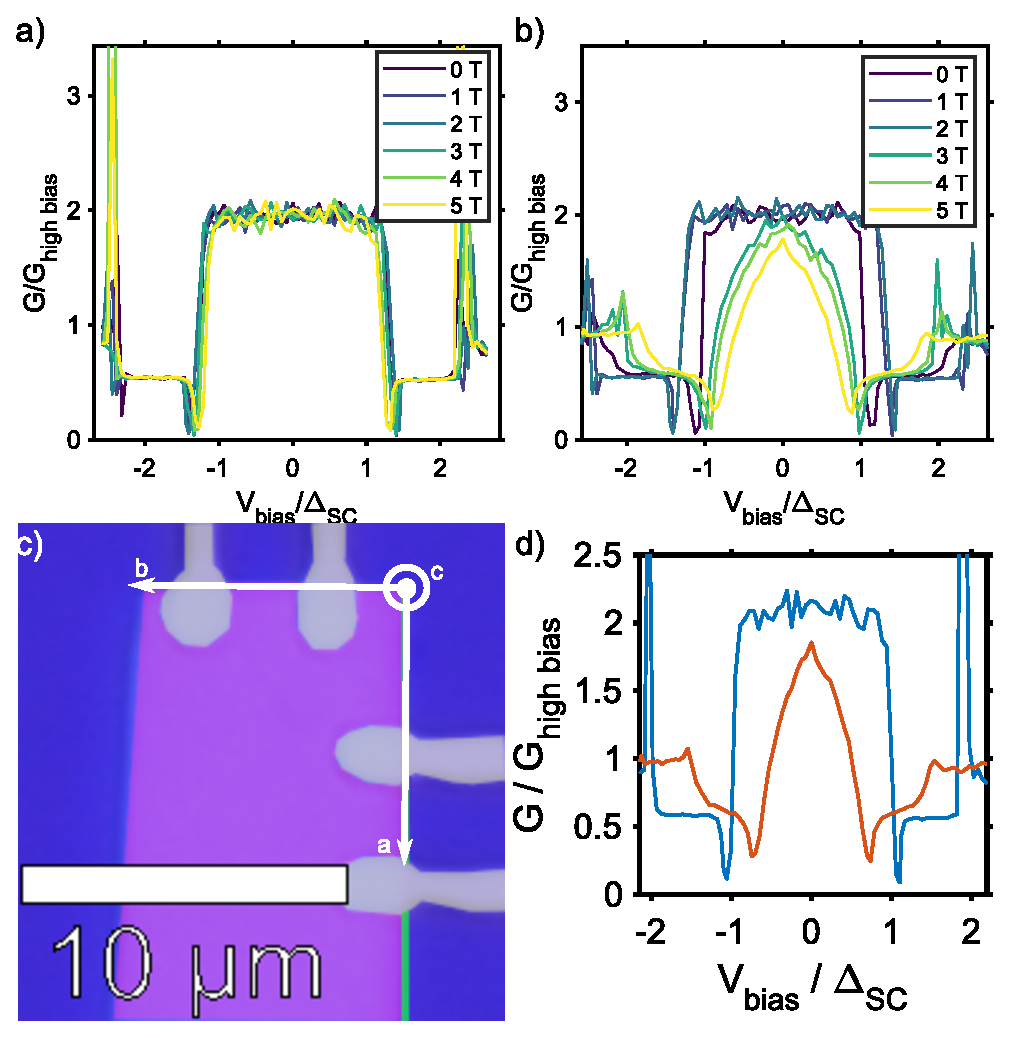
\includegraphics[width = \textwidth]{Chap4/Figures/MagneticField.eps}
    \caption{Caption}
    \label{fig:PARField}
\end{figure}
\section{Conclusion}
In this work we expanded upon the methods used in Chapter \ref{chap:chap3}. When contacting straight, crystallographic edges we observe \acl{PAR} while contacts on ``rough" edges displayed normal \acl{AR} spectra. 
 
\chapter{Conclusion}
\label{chap:conclusion}
\todo{Finish and edit summary}
\section{Summary}
In this dissertation we have presented numerous works investigating the topological nature of iron-based superconductor \acl{FTS}. To probe the topological nature of \ac{FTS} we required a fabrication process that consistently left the surfaces and edges of the crystals in pristine condition. Thus in Chapter II we discussed the concept, development, and optimization of the ``Cleanroom-in-a-Glovebox". This glovebox takes the workflow from a standard cleanroom photolithography process and condenses it into an inert argon environment. The merits of such works were demonstrated by comparing the Raman signals of various air-sensitive materials before and after exposure to air. Furthermore, these materials were subsequently fabricated into electronic devices using the photolithography workflow and shown to have similar quality Raman signals, demonstrating the power of the glovebox fabrication process. The linear layout of the fabrication workflow was optimized to maximize the number of available machines as well as minimize the time between fabrication steps. In addition to powerful fabrication and characterization abilities, the glovebox is also a perfect tool for training the next generation quantum workforce. The simple interfaces of the fabrication facilities provide a low-stress situation for scientists to learn nanofabrication without fear of breaking the equipment. The conveyor-belt layout of the glovebox takes the mental load off of the student-scientists so they can focus on the creative and fun aspects of creating mesoscopic devices.\par
In Chapter III we presented strong evidence for a normal mode that exists purely on the hinge or the side of the \ac{FTS} crystal in the superconducting state. Recent theoretical work has suggested that such a mode could be the result of the combination of an exotic $s^{\pm}$ order parameter and a topological surface state. In short, the anisotropy of the superconducting phase gaps out adjacent faces of the \ac{TI} causing a normal mode at zero energy to appear at the hinge between the top and side surfaces. 
\par
Finally, in Chapter IV we extend the scope of our electronic spectroscopy probe of \ac{FTS} to undercover exciting underlying physics. 

\todo{Finish and edit future work}
\section{Future Work}
Beyond finishing the work put forth in Chapter IV, there is a clear and exciting road forward for \ac{FTS} and other topological superconductors. Here I lay out some experiments I believe would provide interesting insight into the fundamental physics of \ac{FTS}.
\subsection{Fe-based topological superconductivity}
In Chapter IV we touched on the concept of symmetries protecting topologies. This work provided evidence that there is an important symmetry on the [100] face of the \ac{FTS} crystal but it would be useful to elucidate whether this is actually due to the c4 symmetry. Here I suggest performing a series of three-point measurements shown in Chapters III and IV on a variety of crystal facets: specifically on the [100], [110], and [010] facets as these would provide the strongest implication of the c4 symmetry. To accomplish this, one would naturally also need a new fabrication process to cut the exfoliated crystal into pristine edges. Here we suggest either RIE (in the fashion of graphene heterostructure devices), FIB (such as the beautiful devices shown in the work of G. B. Osterhoudt\cite{Osterhoudt2019}), or shadow-mask techniques while growing MBE thin-films.

\startappendices
\appendix{Pseudocode for Andreev Reflection fitting}
\label{app:ARfit}
As mentioned in the main text, \acl{AR} is the process by which an electron is reflected as a hole at the interface between a normal-metal / superconductor interface. By modeling and fitting our data to this model we are able to extract useful quantities such as the superconducting gap size (at a specific temperature), the transparency of the interface, and the thermal broadening of our spectra from our junction size. Thus, here I layout a condensed version of the \ac{BTK} calculation for differential conductance across a normal-metal / superconducting interface then I go through pseudo-code on how to fit this calculation to our data.

\section{BTK Theory}
In 1964, Alexander F. Andreev published a paper describing a process by which an electron incident upon a superconductor forms a cooper pair in the superconductor and retro-reflects a hole\cite{Andreev1964}. This phenomena was originally used to describe the thermal conductivity properties observed in superconductors in the intermediate state where there are many normal sections in direct contact with superconducting sections. It wasn't until 1982 that Blonder, Tinkham, and Klapwijk gave a complete discussion of the phenomena including the effect of the barrier magnitude, a model for the excess current, and predictions for the differential conductance of such a junctions\cite{BTK}.\par

\subsection{The \ac{BdG} Formalism}
The key innovation in the \ac{BTK} model is the use of the \ac{BdG} equations to match the wavefunctions of the quasi-particles excitations at the interface\cite{BTK}. Here I will closely follow the explanation of the \ac{BdG} equations shown in Chapter 14 of "Topological Insulators and Topological Superconductivity" by Bernevig and Hughes\cite{bernevig_hughes_2013}. First we start with the Hamiltonian for a single-particle in a simple metal.
\begin{align}
    H = \left(\frac{p^{2}}{2m}-\mu\right)I_{2\times2}
\end{align}
Where $\mu$ is the chemical potential and $I_{2\times2}$ is the identity matrix in the spin variables. The second-quantized Hamiltonian is given by:
\begin{align}
    H = \sum_{\textbf{p},\sigma}c_{\textbf{p}\sigma}^{\dagger}\left(\frac{p^{2}}{2m}-\mu\right)c_{\textbf{p},\sigma}
\end{align}
Where $c^{\dagger}$ and $c$ are the quasi-particles creation and annihilation operators respectively. Using the anti-commutativity relation of fermions, $\{c_{\textbf{p}\sigma}^{\dagger},c_{\textbf{p}'\sigma'}\}=\delta_{\sigma\sigma'}\delta_{\textbf{p}\textbf{p}'}$, we can rewrite the Hamiltonian above as,
\begin{align}
    H = \frac{1}{2}\sum_{\textbf{p}\sigma}\left[c_{\textbf{p}\sigma}^{\dagger}\epsilon(p)c_{\textbf{p}\sigma}-c_{-\textbf{p}\sigma}\epsilon(-p)c_{-\textbf{p}\sigma}^{\dagger}\right]+\frac{1}{2}\sum_{p}\epsilon(p)
\end{align}
Where $\epsilon(p)\equiv\left(\frac{p^{2}}{2m}-\mu\right)$ and we have relabeled the sum index \textbf{p} in the second term to -\textbf{p}. Here we introduce a new spinor to explicitly label the energy eigenvalues for both spins of both $\epsilon_{p}$ and $\epsilon_{-p}$. E.g., we define $\Psi_{\textbf{p}}\equiv\left(c_{\textbf{p}\uparrow} c_{\textbf{p}\downarrow} c_{-\textbf{p}\uparrow}^{\dagger}c_{-\textbf{p}\downarrow}^{\dagger}\right)$, then we can rewrite the above Hamiltonian as,
\begin{align}
    H &= \sum_{\textbf{p}}\Psi_{\textbf{p}}^{\dagger}H_{BdG}(\textbf{p})\Psi_{\textbf{p}}+\text{constant}\\
    H_{BdG}(\textbf{p}) &= \frac{1}{2}
    \begin{pmatrix}
    \epsilon(p) & 0 & 0 & 0\\
    0 & \epsilon(p) & 0 & 0\\
    0 & 0 & -\epsilon(-p) & 0\\
    0 & 0 & 0 & -\epsilon(-p)
    \end{pmatrix}
\end{align}
The point of this formalism becomes immediately apparent when we introduce a superconducting pairing potential.
\begin{align}
    H_{\Delta} &= \Delta c_{\textbf{p}\uparrow}^{\dagger}c_{-\textbf{p}\downarrow}^{\dagger}+\Delta^{*}c_{-\textbf{p}\downarrow}c_{\textbf{p}\uparrow}\\
    &= \frac{1}{2}\left[\Delta\left(c_{\textbf{p}\uparrow}^{\dagger}c_{-\textbf{p}\downarrow}^{\dagger}-c_{-\textbf{p}\downarrow}^{\dagger}c_{\textbf{p}\uparrow}^{\dagger}\right)+\Delta^{*}\left(c_{-\textbf{p}\downarrow}c_{\textbf{p}\uparrow}-c_{\textbf{p}\uparrow}c_{-\textbf{p}\downarrow}\right)\right]\\
    \therefore H+H_{\Delta} &= \sum_{\textbf{p}}\Psi_{\textbf{p}}^{\dagger}H_{BdG}(\textbf{p},\Delta)\Psi_{\textbf{p}}\\
    H_{BdG}(\textbf{p},\Delta) &= \frac{1}{2}
    \begin{pmatrix}
    \epsilon(p) & 0 & 0 & \Delta\\
    0 & \epsilon(p) & -\Delta & 0\\
    0 & -\Delta^{*} & -\epsilon(-p) & 0\\
    \Delta^{*} & 0 & 0 & -\epsilon(-p)
    \end{pmatrix}
\end{align}
Using this formalism, we can see that the pairing potential simply couples the upper and lower blocks of the $H_{BdG}$ for the simple metal Hamiltonian. From here we can diagonalize $H_{BdG}$ to obtain the energy eigenvalues.
\begin{align}
    E_{\pm} = \pm\sqrt{\epsilon(\textbf{p})^{2}+|\Delta|^{2}}
\end{align}
The quasi-particles dispersion relations for the normal metal $(|\Delta|=0)$ and the superconductor $(|\Delta|=0.1m)$ are plotted in Fig \ref{fig:AndreevDiagram} which also conveniently serves as a perfect starting point for the discussion of the \ac{BTK} calculation.\par

\begin{figure}
    \centering
    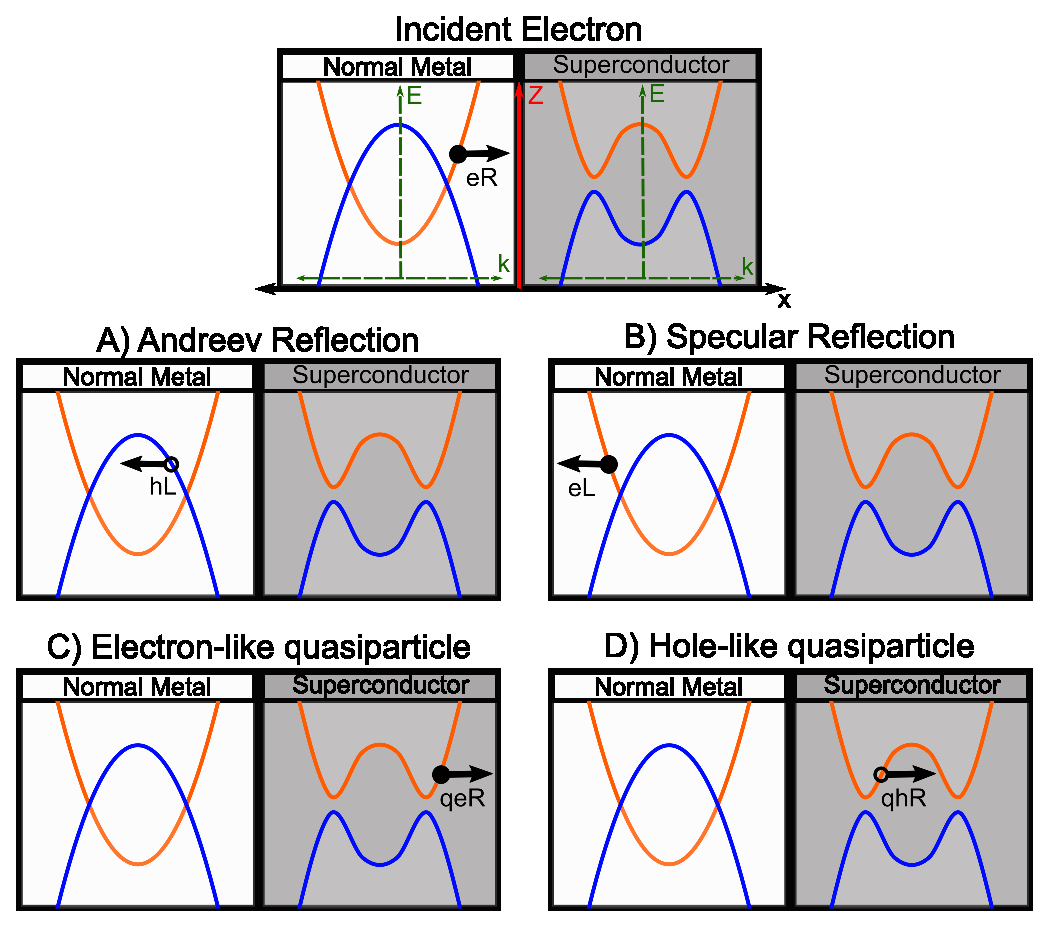
\includegraphics[width=\textwidth]{Appendices/Figures/AndreevDiagram.eps}
    \caption{Dispersion relations for a normal metal and superconductor in physical contact with one another. The red axis denotes the real-space position of the two materials with a potential barrier at their interface. The subset green, dashed axes denote the dispersion relations within the respective materials. A right-moving incident electron (top) can take one of four paths once it hits the NM/SC barrier: A) Andreev reflect as a left-moving hole, B) Normally reflect as a left-moving electron, C) Transmit as a right-moving electron-like quasi-particles, or D) Transmit as a right-moving hole-like quasi-particles.}
    \label{fig:AndreevDiagram}
\end{figure}

\subsection{The \ac{BTK} calculation}
First, we consider a normal metal in contact with a superconductor. The dispersion relations for the two are as calculated in the previous section and the barrier in the interface is modeled by a Dirac-delta function with magnitude $Z$. \ac{BTK} considers a plane-wave electron incident from the normal metal on the left side of the junction thus when the electron encounters the barrier there are four possibilities (shown in Fig \ref{fig:AndreevDiagram}):\\
\\
A) The electron is Andreev reflected as a left-moving hole and a right-moving Cooper-Pair transmits into the superconducting fluid.\\
B) The electron is specularly reflected as a left-moving electron.\\
C) The electron is transmitted as a right-moving electron-like quasiparticle.\\
D) The electron is transmitted as a right-moving hole-like quasiparticle.\\
\\
To solve for the probabilities of each process occurring we first define the momenta in the normal metal and superconductor respectively as,
\begin{align}
    k^{\pm} &= \sqrt{\frac{2m_N}{\hbar^{2}}}\sqrt{E_{FN}\pm E}\\
    q^{\pm} &= \sqrt{\frac{2m_{SC}}{\hbar^{2}}}\sqrt{E_{FSC}\pm\sqrt{E^{2}-\Delta^{2}}}
\end{align}
Then we simply match the boundary conditions, i.e., the wavefunctions and their derivatives are the same at the boundary. Starting with the wavefunctions,
\begin{align}
    \begin{pmatrix}1\\0\end{pmatrix}e^{ik^{+}x_{0}}
    + C\begin{pmatrix}1\\0\end{pmatrix}e^{-ik^{+}x_{0}}
    + D\begin{pmatrix}0\\1\end{pmatrix}e^{ik^{-}x_{0}}
    =
    A\begin{pmatrix}u_{0}\\v_{0}\end{pmatrix}e^{iq^{+}x_{0}}
    + B\begin{pmatrix}u_{0}\\v_{0}\end{pmatrix}e^{-iq^{-}x_{0}}
\end{align}
then the derivatives.
\begin{align}
    &\frac{\hbar^{2}}{2m_{N}}\left\{
    ik^{+}\begin{pmatrix}1\\0\end{pmatrix}e^{ik^{+}x_{0}}
    -ik^{+}C\begin{pmatrix}1\\0\end{pmatrix}e^{-ik^{+}x_{0}}
    +ik^{-}D\begin{pmatrix}1\\0\end{pmatrix}e^{ik^{-}x_{0}}
    \right\}\\
    &= \frac{\hbar^{2}}{2m_{SC}}\left\{
    iq^{+}A\begin{pmatrix}u_{0}\\v_{0}\end{pmatrix}e^{iq^{+}x_{0}}
    -iq^{-}B\begin{pmatrix}u_{0}\\v_{0}\end{pmatrix}e^{-iq^{-}x_{0}}
    \right\}\\
    &\qquad+H*\left\{
    A\begin{pmatrix}u_{0}\\v_{0}\end{pmatrix}e^{iq^{+}x_{0}}
    +B\begin{pmatrix}u_{0}\\v_{0}\end{pmatrix}e^{-iq^{-}x_{0}}
    \right\}
\end{align}
where $x_{0}$ is the position of the barrier (it is typically set to zero) and $u_{0}$, $v_{0}$ are the electron-weight and hole-weight of the quasiparticles, respectively. Thus the transmission coefficients are given by:
\begin{align}
    \begin{matrix}
    a=\left(\left|A\right|^{2}*\left(u_{0}^{2}-v_{0}^{2}\right)\right)\frac{q_{SC}^{+}}{k_{N}^{+}} & b=\left|B\right|^{2}*\left(u_{0}^{2}-v_{0}^{2}\right)\frac{q_{SC}}{k_{N}^{+}}\\
    c = \left|C\right|^{2} & d = \left|D\right|^{2}*\frac{k_{N}^{-}}{k_{N}^{+}}
    \end{matrix}
\end{align}

Before plugging in the momentum values there are some quick simplification we can make here to improve readability. Using, $v_{F}^{SC}=\hbar k_{FSC}/m_{SC}$ and $v_{FN}=\hbar k_{FN}/m_{N}$, we define $Z_{0}\equiv H/\hbar\sqrt{v_{FN}*v_{SC}}$. Now we can define the $Z$ parameter that will characterize the potential barrier as:
\begin{align}
    Z^{2}&\equiv Z_{0}^{2}+\frac{(1-r_{v}^{2})}{4r_{v}}\\
    r_{v}&\equiv\frac{v_{FN}}{v_{FSC}}=\sqrt{\frac{E_{FN}m_{SC}}{E_{FSC}m_{N}}}
\end{align}
so that we can set $E_{FN}=E_{FSC}$ and $m_{N}=m_{SC}$. Next, we set $\gamma=u_{0}^{2}+(u_{0}^{2}-v_{0}^{2})Z^{2}$. Finally, we note that the solution is vastly different in the two scenarios where $E<\Delta$ and $E>\Delta$ thus it behooves us to write them as a piece-wise function.
\begin{align}
    \begin{matrix}
    a(E)=\begin{cases}
    0 & E<\Delta\\
    \frac{(u_{0}^{2}-v_{0}^{2})u_{0}^{2}(1+Z^{2})}{\gamma^{2}} & E\geq\Delta\end{cases} &
    b(E)=\begin{cases}
    0 & E<\Delta\\
    \frac{(u_{0}^{2}-v_{0}^{2})v_{0}^{2}Z^{2}}{\gamma^{2}} & E\geq\Delta
    \end{cases}\\
    c(E)=\begin{cases}
    \frac{4Z^{2}(1+Z^{2})(\Delta^{2}-E^{2})}{E^{2}+(\Delta^{2}-E^{2})(1+2Z^{2})^{2}} & E<\Delta\\
    \frac{(u_{0}^{2}-v_{0}^{2})Z^{2}(1+Z^{2}}{\gamma^{2}} & E\geq\Delta
    \end{cases} &
    d(E)=\begin{cases}
    \frac{\Delta^{2}}{E^{2}+(\Delta^{2}-E^{2})(1+2Z^{2})^{2}} & E<\Delta\\
    \frac{u_{0}^{2}v_{0}^{2}}{\gamma^{2}} & E\geq\Delta
    \end{cases}
    \end{matrix}
\end{align}
Thus we can simply read-off the differential conductance across the junction as:
\[
\sigma = 2*d(E)+a(E)+b(E)
\]
The plots for various potential barrier strengths ($Z$) are shown in Fig \ref{fig:BTKGraphs} along with some other corrections in the next section.

\section{Pseudo-Code for fitting spectra}
Tunneling in a normal metal/superconductor interface can produce wildly different spectra depending on the various parameters such as temperature, barrier height, disorder, and more. This pseudo-code was written to characterize such superconducting tunneling spectra via the 1D \ac{BTK} model and extract information such as the superconducting gap. The results of running each individual algorithm are shown in Fig \ref{fig:BTKGraphs} to show how each parameters affects a tunneling spectrum, however in most cases one will need to use two or more of these algorithms in concert to obtain a good fit for a spectrum. For a full extension of the model to 2D, 3D, and unconventional superconductivity please read the in-depth topical reviews by D. Daghero \& R. S. Gonnelli\cite{Daghero2010} and Kashiwaya \& Tanaka\cite{Kashiwaya2000}.\par
First we write a function (Algorithm 1) that calculates the \ac{BTK} conductance spectra at zero temperature. The inputs to this functions are: the measured voltage vector in millivolts (meV), the barrier height (Z), the superconducting energy gap ($\Delta_{SC}$), and the thermal broadening parameter ($\Gamma$).
\begin{figure}
    \centering
    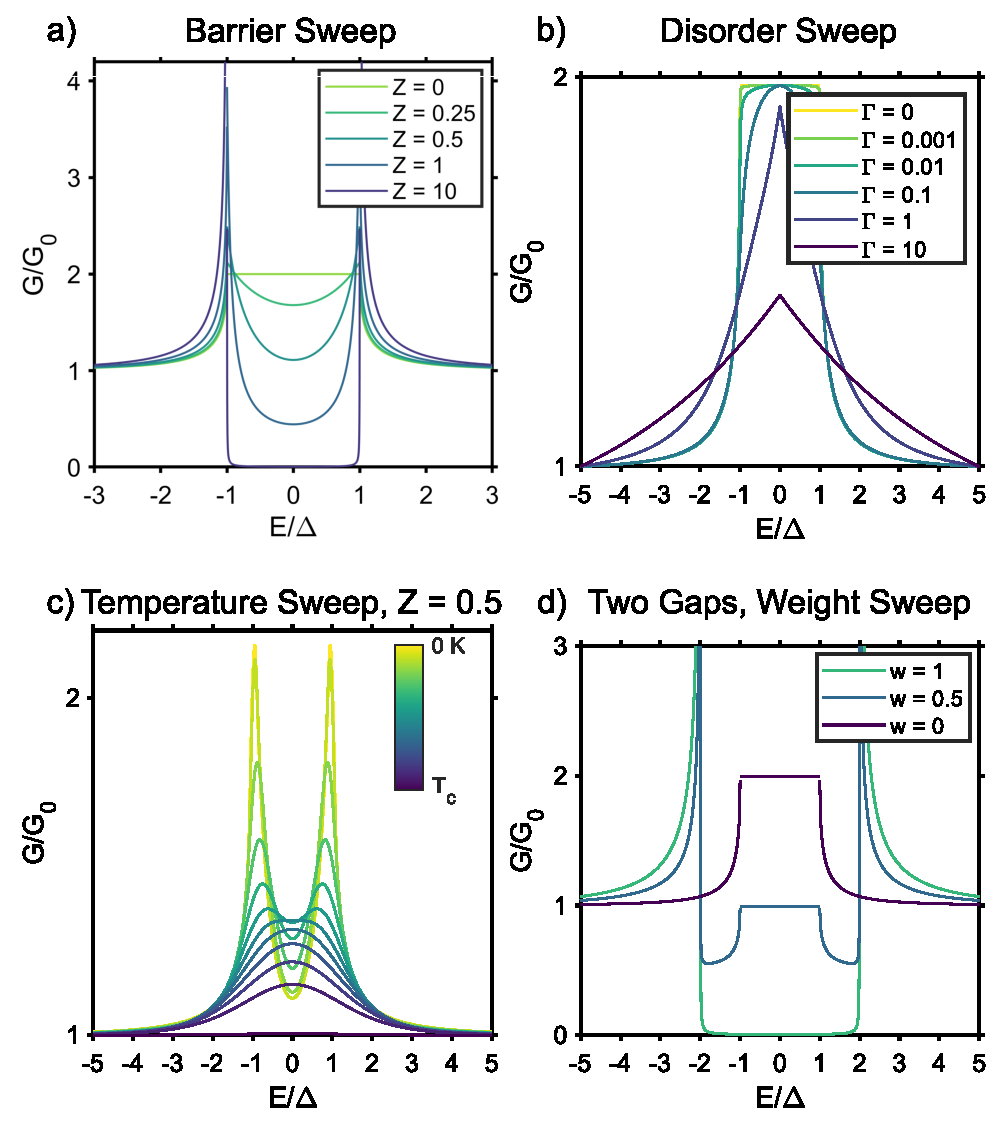
\includegraphics[width=\textwidth]{Appendices/Figures/BTKCalculations.eps}
    \caption{Various demonstrations of the differential conductance calculated using the algorithms described in A.2. a) Single gap, zero Kelvin sweep of the potential barrier strength $Z$. b) Single gap, zero Kelvin, zero barrier sweep of the thermal broadening parameter $\Gamma$. c) Single gap, half-strength barrier, temperature sweep. d) Two superconducting gaps where the second gap is twice as large as the first demonstrating the $w$ parameter in action.}
    \label{fig:BTKGraphs}
\end{figure}
\begin{algorithm}
\caption{Single Gap \ac{BTK} conductance}\label{zeroT}
\begin{algorithmic}[1]
\Function{BTK1g}{$meV, Z, \Delta_{SC}, \Gamma$}\Comment{Returns conductance vector.}
\State $N_{q}=\left|\frac{meV+i\Gamma}{\sqrt{(meV+i\Gamma)^{2}-\Delta_{SC}^{2}}}\right|$\Comment{quasi-particles \ac{DoS}}
\State $N_{p}=\frac{\Delta_{SC}}{\sqrt{(meV+i\Gamma)^{2}-\Delta_{SC}^{2}}} $\Comment{Pair \ac{DoS}}
\State $\tau_{n} = \frac{1}{1+Z^{2}}$\Comment{Define the transparency}
\State $\gamma = \frac{N_{q}-1}{N_{p}}$\Comment{Define $\gamma$ function. Not $\Gamma$!}
\State $G = \frac{1+\tau_{n}\left|\gamma\right|^{2}+\left(\tau_{n}-1\right)\left|\gamma^{2}\right|^{2}}{\left|1+\left(\tau_{n}-1\right)\gamma^{2}\right|^{2}}$\Comment{G will be a vector.}
\State \textbf{return} $G$, $\tau_{n}$\Comment{We return $\tau_{n}$ in preparation for the next function.}
\EndFunction
\end{algorithmic}
\end{algorithm}
This code is useful for understanding what the conductance looks like at various Z-values, Gap-sizes. The broadening term can be used (or fit) to simulate a finite temperature since (as the name suggests) it is basically a term that broadens the spectral peaks out.\par
If we want to incorporate the temperature in a more rigorous way we can take the outputs of the previous function then integrate the convolution of their product with the Fermi function (Algorithm 2).
\begin{algorithm}
\caption{BTK at finite temperature}
\begin{algorithmic}[1]
\State $G, \tau_{n} = BTK1g(meV, Z, \Delta_{SC}, \Gamma)$
\For{V in meV}
\State $f_{C} = G\tau_{n}\left(\frac{1}{e^{\left(e-V\right)/k_{b}T}}-\frac{1}{e^{E/k_{b}T+1}}\right)$\Comment{Convolution. Outputs a function.}
\State $I_{ns}(V) = \int_{-\infty}^{\infty}f_{C}dE$\Comment{Integrate function over all energies.}
\EndFor
\State $\frac{dI}{dV} = \left|\nabla(I_{NS})\right|$
\end{algorithmic}
\end{algorithm}
I've used an anonymous function since these codes were originally written in MatLab however the same task can be accomplished in Python with a lambda function instead. Alternatively, one could also skip the for-loop by implementing the numpy function numpy.convolve(vector1,vector2). Algorithm 3 is a simple extension that allows us to model the conductance with two superconducting gaps.\par
\begin{algorithm}
\caption{Two Gap BTK Fit}{BTK\_2Gap}
\begin{algorithmic}
\State $G_{1},\tau_{1} = BTK\_at\_finite\_temperature(meV,Z_{1},\Delta_{SC,1},\Gamma_{1})$
\State $G_{2},\tau_{2} = BTK\_at\_finite\_temperature(meV,Z_{2},\Delta_{SC,2},\Gamma_{2})$
\State $G = w*G_{1} + (w-1)*G_{2}$\Comment{$w$ ranges between 0 and 1.}
\end{algorithmic}
\end{algorithm}
Algorithm 4 is another simple function to either fit the temperature-dependence of the gaps to what's predicted via \ac{BCS} theory or use this function to generate a series of gap sizes for our \ac{BTK} versus temperature function later. I've presented this as a function so that it's easier to fit with, but this can be defined as an anonymous function (MatLab) or lambda function (Python) to reduce file complexity. 
\begin{algorithm}
\caption{BCS Gap}\label{euclid}
\begin{algorithmic}[1]
\Function{BCSGap}{$T$,$\Delta_{0},T_{c}$,$\alpha$}\Comment{SC gap at temperature T.}
\State $\Delta(T) = \left|1.74k_{b}T_{c}\left(1-\left(\frac{T}{T_{c}}\right)\right)^{\alpha}\right|$
\State \textbf{return} $\Delta(T)$
\EndFunction
\end{algorithmic}
\end{algorithm}
Finally Algorithm 5 denotes the whole script for modelling and plotting a range of temperatures to both single gap and two-gap BTK models using the above functions. Fitting the function varies by platform a bit but the pseudo-code is to define the ``BTK and finite temperature" file as the model as use the built-in fit functions.
\begin{algorithm}
\caption{BTK Temperature Fit}{BTKTempFit}
\begin{algorithmic}[1]
\State $Temps, dataCell = loadData(folder)$\Comment{``load\_data" is a script written by G. Osterhoudt.}
\State $fig = figure(1)$\Comment{Can use plt.subplot in Python}
\State $G_{0} = zeros(length(Temps))$\Comment{Will populate with normalization.}
\State $j = 0$\Comment{Iteration variable}
\For{T in Temps}
\State $\Delta_{SC} = BCSGap(T,\Delta_{0},T_{c},\alpha)$
\State $G = BTK\_at\_finite\_temperature(meV, Z, \Delta_{SC}, \Gamma)$
\State $Smooth$
\State $G_{0}(j) = G(end)$
\State $j += 1$
\State $plot(meV, G/G_{0})$
\EndFor
\end{algorithmic}
\end{algorithm}
 
\appendix{Model of the differential conductance circuit}
\label{app:Circuit}
As discussed in Chapter III, we are interested in measuring the differential conductance of samples versus a DC bias voltage. This is because the differential conductance of a normal sample is directly proportional to the \ac{DoS} of a material. To see this, let's start off by considering the contribution of a single carrier tunneling from our contact to the sample, we also must consider carriers tunneling from the sample to the contact:
\begin{align}
    i_{sample \rightarrow contact} = -2e\frac{2\pi}{\hbar}|M|^{2}\left(\rho_{s}\left(\varepsilon\right)\cdot f\left(\varepsilon\right)\right)\cdot\left(\rho_{c}\left(\varepsilon-eV\right)\cdot\left[1-f\left(\varepsilon-eV\right)\right]\right)\\
    i_{contact \rightarrow sample} = -2e\frac{2\pi}{\hbar}|M|^{2}\left(\rho_{c}\left(\varepsilon-eV\right)\cdot f\left(\varepsilon-eV\right)\right)\cdot\left(\rho_{s}\left(\varepsilon\right)\cdot\left[1\cdot f\left(\varepsilon\right)\right]\right)
\end{align}
Where $|M|^2$ is the tunneling matrix element which describes the specifics of the junction (for an excellent breakdown of how this matrix function corresponds to different junction types see Berthod (2011)\cite{Berthod2011}), $\rho_{s,c}$ is the \ac{DoS} of the sample and contact respectively, and $f(\varepsilon)$ is the Fermi function. To get the total current across this junction we sum the contribution from both directions and integrate over all energies.
\begin{align}
    I = -\frac{4\pi e}{\hbar}\int_{-\infty}^{\infty}|M|^{2}\rho_{s}\left(\varepsilon\right)\rho_{c}\left(\varepsilon-eV\right)\left[f\left(\varepsilon\right)\cdot\left[1-f\left(\varepsilon-eV)\right]\right]-f(\varepsilon-eV)\cdot\left[1-f(\varepsilon\right)\right]d\varepsilon
\end{align}
Here we take the derivative with respect to $\varepsilon$ to get:
\begin{align}
    \frac{dI}{d\varepsilon} = -\frac{4\pi e}{\hbar}|M|^{2}\rho_{s}\left(\varepsilon\right)\rho_{c}\left(\varepsilon-eV\right)\left[f\left(\varepsilon\right)\cdot\left[1-f\left(\varepsilon-eV)\right]\right]-f(\varepsilon-eV)\cdot\left[1-f(\varepsilon\right)\right]
\end{align}
Thus at a given bias voltage (eV) and temperature the differential conductance is proportional to the product of the densities of states of the sample and contact. Therefore if the contact has a constant \ac{DoS} in energy, the differential conductance is directly proportional to the \ac{DoS} of the sample.\par
When probing a sample in the superconducting state, the differential conductance can be used to probe the superconducting characteristics of the system. As an example, the \ac{BTK} theory discussed in Appendix A demonstrates how to use the differential conductance versus bias voltage curve to determine the magnitude of the superconducting energy gap.

\section{Measuring differential conductance}
One method of measuring the differential conductance is to measure the current-voltage characteristics and then take a numerical derivative. This can be time-consuming to get enough data to ensure a low-noise $\frac{dI}{dV}$ curve and can lead to resolution limitations. An alternate method is to add a small AC voltage on top of the DC voltage then measure the resulting AC current. In this case, we can express the current response as a Taylor series:
\begin{align}
    I(V+v\cos(\omega t)) = I(V) + \frac{dI}{dV}v\cos(\omega t) + \frac{1}{2}\frac{d^{2}I}{dV^{2}}v^{2}\cos^{2}(\omega t) + \dots
\end{align}
Thus the signal measured at frequency $\omega$ will be proportional to the first derivative of the current-voltage characteristics. We can therefore use a \ac{LIA} to directly measure the differential conductance without any numerical processing. Then we can probe the \ac{DoS} for a range of the band structure by sweeping the bias voltage and measuring the $\frac{dI}{dV}$ at every point.\par

\section{Circuit construction}
Now let's see how this model is executed in the lab by examining the AC + DC adder circuit in more detail. The circuit as of May 2021 is shown in \ref{fig:Circuit}. As we are interested in measuring the bias voltage across the junction (rather than the bias current) we start by sending in a DC voltage (point A) with a BK Precision 1785b. Given that this power supply only has 10 mV resolution and that the spectroscopic features we are searching for are of order 1 mV, we need to use a voltage divider (point B). This voltage divider introduces some problems that will be discussed in the next section. The AC voltage is then added to the DC voltage via a one-to-one transformer (point C) which has the added benefits of isolating the AC signal from the rest of the circuit. The AC signal can be sent through an attenuating circuit first if the current is too large. To find the current going through the sample we either insert a resistor in series with the sample or use a current pre-amplifier (pre-amp) but in both cases, the AC and DC voltages over the resistor (or output from the pre-amp) are measured in parallel (point E). The current going through the sample is then simply the measured voltage divided by the resistor (or 1/sensitivity if using the pre-amp). We also measure the AC and DC voltages at the sample so that we do not need to assume the voltages we output are actually what is placed across the sample (point D).\par
\begin{figure}
    \centering
    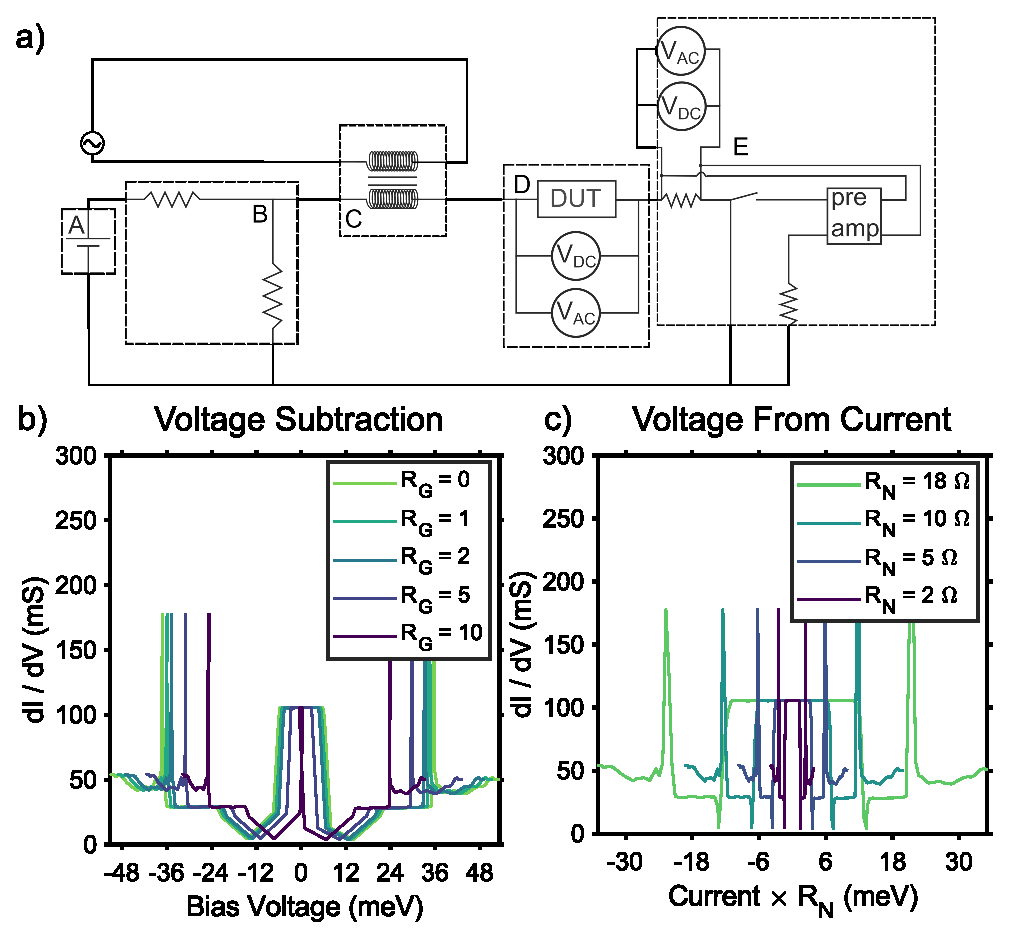
\includegraphics{Appendices/Figures/Circuit.eps}
    \caption{a) Circuit diagram to add AC and DC voltages then measure differential conductance as a function of applied DC bias. b) Voltage correction of data in Chapter \ref{chap:PAR} via subtraction of extra measured voltage due to the system resistances along the way. c) Voltage correction of the same data by measuring the resulting current and multiplying it by the normal resistance.}
    \label{fig:Circuit}
\end{figure}

\subsection{Circuit troubles and solutions}
The SR-570 Low Noise Current Preamplifier was found to send out a large voltage spike ($\sim$ 1V!) across the circuit when switching sensitivities, which often damaged or destroyed the device. For this reason we switched to using the resistor method. For higher resistance devices in which a pre-amp is needed to measure a much smaller current it is recommended that the user ground the device, disconnect the pre-amp, make the gain and sensitivity adjustments, then reconnect and unground the device. This is a slow process but it will ensure the pre-amp voltage spike does not damage the device under test.\par
The governing physics behind the voltage divider is shown in the equation,
\begin{align}
    V_{out} = V_{in}*\frac{R_{2}}{R_{1}+R_{2}}
\end{align}
however this model assumes that the output voltage is over an open circuit meaning that the resistance of the sample is large compared to $R_{2}$. When samples have a small resistance, the output voltage can change drastically from the expected value. This is especially concerning when the resistance of a sample changes drastically over a single measurement as can be the case when measuring superconducting tunneling. One solution is to use commercial voltage regulators to ensure a steady voltage is maintained even at high currents. However, most of these commercial voltage regulators have a minimum voltage output around 1.2 V which is three orders of magnitude larger than our 1 mV resolution requirement. Another solution is to switch to current-biased measurements when dealing with low-resistance samples however converting back to bias voltage can be quite tricky as will be discussed in the next section. Lastly would be to simply use a commercial high-resolution DC voltage source such as the DC205 DC Voltage Source from SRS in order to eliminate the voltage divider completely. These sources can be quite expensive but offer resolutions down to the $\mu$V level.\par 

\section{Three-point measurements}
Lastly, I would like to discuss some peculiarities with the three-point measurements used in Chapters III \& IV. In particular, since we use the measured voltage across the junction as our bias voltage (independent axis) we need to carefully consider what voltage is actually being applied across the relevant part of the junction. To illustrate, the reason a four-probe (Kelvin) measurement is preferred when determining a sample's resistivity is the Kelvin resistance does not include contact resistance\cite{Kuphaldt2015}. However in our measurement the quantity that we are measuring \textit{is} the contact resistance thus we want to be sure we don't split that resistance out of our measurement. This presents an issue as the resistance of the chrome/gold contacts will also stay in the measurement and add additional voltage to our bias voltage reading. There are two ways to correct for this: 1) Use the resistivity of a control chrome/gold device to subtract out the resistance (and voltage) or 2) convert the measured current back to a voltage by multiplying by the normal state resistance of the junction. The results of both correct are shown below for varying values of gold resistance.

%%%%%%%%%%%%%%%%%%%%%%%%%%%%%%%%%%%%%%%%%%%%%%%%%%%%%%%%%%%%%%%%%%%%%%%%%%%%%%%%%%%%%%%%%%%%%
%%%%%%%%%%%%%%%%%%%%%%%%%%%%%%%%%%%%%%%%%%%%%%%%%%%%%%%%%%%%%%%%%%%%%%%%%%%%%%%%%%%%%%%%%%%%%
%%%%%%%%%%%%%%   BIBLIOGRAPHY %%%%%%%%%%%%%%%%%%%%%%%%%%%%%%%%%%%%%%%%%%%%%%%%%%%%%%%%%%%%%%%%
%%%%%%%%%%%%%%%%%%%%%%%%%%%%%%%%%%%%%%%%%%%%%%%%%%%%%%%%%%%%%%%%%%%%%%%%%%%%%%%%%%%%%%%%%%%%%
%%%%%%%%%%%%%%%%%%%%%%%%%%%%%%%%%%%%%%%%%%%%%%%%%%%%%%%%%%%%%%%%%%%%%%%%%%%%%%%%%%%%%%%%%%%%%
\startbibliography
\begin{singlespace}
    \printbibliography[heading = none]
\end{singlespace}

\end{document}